%%%%%%%%%%%%%%%%%%%%%%%%%%%%%%%%%%%%%%%%%%%%%%%%
\input{./format/preamble.ltx} 

%%%%%%%%%%%%%%%%%%%%%%%%%%%%%%%%%%%%%%%%%%%%%%%%
% as needed, comment the following lines by prefixing the percent sign (%) at the start of the line

\Drafttrue % comment to disable putting some guides in the draft form of the document

\PutLineNumberstrue % comment to disable line numbers and certain  preparation guides 

\Figurestrue % comment to disable the rendering figures

\GroupIDtrue % comment to disable group ID

\ResultDiscusstrue % comment to disable results and discussions

\Conctrue % comment to disable conclusions

%\Finishedtrue % comment to disable manuscript for final defense or binding/submission

%\ApprovalSheetSignedtrue % comment to disable inclusion of the signed approval sheet

%\Gradtrue % comment to disable graduate school format

%\PhDtrue % comment to disable PhD dissertation format

%\PubListtrue % comment to disable publication list

\Vitatrue % comment to disable author(s) vita

\Indextrue % comment to disable index 

%%%%%%%%%%%%%%%%%%%%%%%%%%%%%%%%%%%%%%%%%%%%%%%%
% document IDs

% specify if dissertation, thesis, project, dissertation proposal, thesis proposal, project proposal 
%\newcommand{\documentType}{Thesis} 
\newcommand{\documentType}{Thesis Proposal}
%\newcommand{\documentType}{Dissertation Proposal}
%\newcommand{\documentType}{Dissertation}
\newcommand{\college}{Gokongwei College of Engineering}
\newcommand{\department}{Department of Electronics and Computer Engineering} 
\newcommand{\degreeType}{Bachelor of Science}
%\newcommand{\degreeType}{Bachelor and Master of Science}  
%\newcommand{\degreeType}{Master of Engineering Program} 
%\newcommand{\degreeType}{Master of Science} 
%\newcommand{\degreeType}{Doctor of Philosophy} 
\newcommand{\degree}{Electronics and Communications Engineering}
\newcommand{\degreeAbbrv}{BS-ECE}
%\newcommand{\degreeAbbrv}{BS-MS-ECE}
%\newcommand{\degreeAbbrv}{MEP-ECE}
%\newcommand{\degreeAbbrv}{MS-ECE}
%\newcommand{\degreeAbbrv}{PhD-ECE}

\newcommand{\documentAdviserTitle}{Dr.} 
\newcommand{\documentAdviser}{Shin C. Maxwell}

\newcommand{\examinerChairTitle}{Dr.} 
\newcommand{\examinerChair}{Amado Z. Hernandez}

% Sort in alphabetically ascending manner the surnames of the examiners
\newcommand{\examinerATitle}{Dr.} 
\newcommand{\examinerA}{Jose Y. Alonzo}

\newcommand{\examinerBTitle}{Dr.} 
\newcommand{\examinerB}{Mariana X. Mercado}

% Note that \examinerC and \examinerD only applies for PhD dissertations
\newcommand{\examinerCTitle}{Dr.} 
\newcommand{\examinerC}{Rafael W. Sison}

\newcommand{\examinerDTitle}{Dr.} 
\newcommand{\examinerD}{Apolinario V. Valenzuela}

% College signatories for graduate theses/dissertations
\newcommand{\RASDTitle}{Dr.} 
\newcommand{\RASDName}{Isabella S. Garcia}

\newcommand{\deanTitle}{Dr.} 
\newcommand{\deanName}{Diego U. Lopez}

\newcommand{\groupID}{ESG-04} % group ID is for undergraduates as of this formatting

\newcommand{\numberOfAuthors}{5} % adapt the number of names below accordingly and sort the sunames in alphabetically ascending manner, like in the following example

\defineAuthor{surname1}{dela Cruz}
\defineAuthor{firstname1}{Juan Z.}

\defineAuthor{surname2}{Franco}
\defineAuthor{firstname2}{Nat Y.}

\defineAuthor{surname3}{Garcia}
\defineAuthor{firstname3}{Sebastian X.}

\defineAuthor{surname4}{Martinez}
\defineAuthor{firstname4}{Isabella W.}

\defineAuthor{surname5}{Rianzares}
\defineAuthor{firstname5}{Max V.}

\newcommand{\documentTitle}{Electrical, Electromagnetic, and Optical Characterization of the InP/InGaAs~Alloy~System} % put tilde (~) between words to indicate non-breaking adjacent words

\newcommand{\keywords}{alloy system, characterization, InP, InGaAs (see IEEE Taxonomy and Thesaurus)}

\newcommand{\finalDefenseDate}{\usdate\today} % replace ''\usdate\today'' by your final defense date; you may need to use non-breaking space with the use of tildes (~); if so, do not remove the tildes in order to not break the date

\ifGrad
\newcommand{\scannedApprovalSheetFileName}{./figure/Signed_Thesis_Approval_Sheet_Graduate.pdf} % filename of the signed approval sheet (for graduate)
\else	
\newcommand{\scannedApprovalSheetFileName}{./figure/Signed_Thesis_Approval_Sheet_Undergraduate.pdf} % filename of the signed approval sheet (for undergraduate)
\fi

\hyphenation{op-tical net-works semi-conduc-tor evi-dent re-la-tive re-si-den-tial po-la-ri-za-tion so-lu-tion/s} % for correcting bad hyphenation

%%%%%%%%%%%%%%%%%%%%%%%%%%%%%%%%%%%%%%%%%%%%%%%%
\input{./format/postamble.ltx} 

%%%%%%%%%%%%%%%%%%%%%%%%%%%%%%%%%%%%%%%%%%%%%%%%
% for placing user-defined-ambles

\DeclareMathAlphabet{\mathitbf}{OML}{cmm}{b}{it} % for math italic bold, but can also use \mathbfit
\newcommand{\redtx}[1]{\textcolor[rgb]{0.65,0.16,0}{#1}} % for formatting text to have a red color
\newcommand{\graytx}[1]{\textcolor[rgb]{0.75,0.75,0.75}{#1}} % for formatting text to have a gray color

%%%%%%%%%%%%%%%%%%%%%%%%%%%%%%%%%%%%%%%%%%%%%%%%
% \includeonly{} is for specifying which files to include; if you only want to work on one or few chapters, you can only include those chapters, which will speed up the document build; advantage: fast if you have a large number of images in your results chapter, which you do not need when you are working on other chapters; you can still reference all the figures in the omitted chapter, as long as you have previously LaTeX-built the entire document

% Note that the file names below must correspond to those names inside \include{} in the \begin{document} ... \end{doument} enviroment, otherwise the chapter will not be included

%  the excludeonly package provides the logically opposite command: \excludeonly{<file list>}

\includeonly{% just comment those portions that you do not want to be included in the parsing
	introduction,
	literature_review,
	theoretical_considerations,
	design_considerations,
	methodology,
	results_and_discussions,
	conclusions,
	answers_to_questions,
	revisions_to_the_proposal,
	revisions_to_the_final,
	usage_examples,
	publication,
	vita,
}

%%%%%%%%%%%%%%%%%%%%%%%%%%%%%%%%%%%%%%%%%%%%%%%%
\begin{document}
\pagenumbering{roman} % roman page numbering starts here

%%%%%%%%%%%%%%%%%%%%%%%%%%%%%%%%%%%%%%%%%%%%%%%%
\input{./format/pre_toc.ltx}
\cleardoublepage

%%%%%%%%%%%%%%%%%%%%%%%%%%%%%%%%%%%%%%%%%%%%%%%%
\begin{SingleSpace}
	\tableofcontents
	\cleardoublepage

	%%%%%%%%%%%%%%%%%%%%%%%%%%%%%%%%%%%%%%%%%%%%%%%%
	\listoffigures
	\cleardoublepage

	%%%%%%%%%%%%%%%%%%%%%%%%%%%%%%%%%%%%%%%%%%%%%%%%
	\listoftables
	\cleardoublepage

	%%%%%%%%%%%%%%%%%%%%%%%%%%%%%%%%%%%%%%%%%%%%%%%
	\phantomsection
	\addcontentsline{toc}{chapter}{Abbreviations and Acronyms}
	{
		\printterms[database=abbreviation, style=indexalign, prelocation=dotfill, location=first, columns=1, postname=\hspace{3em}]
		\thispagestyle{plain}
	}
	\cleardoublepage

	%%%%%%%%%%%%%%%%%%%%%%%%%%%%%%%%%%%%%%%%%%%%%%%
	\phantomsection
	\addcontentsline{toc}{chapter}{Notations}
	{
		\printterms[database=notation, style=indexalign, prelocation=dotfill, location=first, columns=1, postname=\hspace{3em}]
		{
			\vspace{3ex}
			\noindent Throughout this \MakeTextLowercase{\documentType}, mathematical notations conform to ISO~80000-2 standard, e.g., variable names are printed in italics, the only exception being acronyms like, e.g., $\mathrm{SNR}$, which are printed in regular font.  Constants are also set in regular font like $\mathrm{j}$.  Standard functions and operators are also set in regular font, e.g., in $\sin \left( \cdot \right)$, $\max \{ \cdot \} $.  Commonly used notations are $t$, $f$, $\mathrm{j} = \sqrt{-1}$, $n$ and $\exp \left( \cdot \right)$, which refer to the time variable, frequency variable, imaginary unit, $n$th variable, and exponential function, respectively.
		}
		\thispagestyle{plain}
	}
	\cleardoublepage

	%%%%%%%%%%%%%%%%%%%%%%%%%%%%%%%%%%%%%%%%%%%%%%%%
	\phantomsection
	\addcontentsline{toc}{chapter}{Glossary}
	{
		\printterms[database=glossary, style=indexalign, prelocation=none, location=hide, columns=1, postname=\hspace{3em}]
		\thispagestyle{plain}
	}
	\cleardoublepage

	%%%%%%%%%%%%%%%%%%%%%%%%%%%%%%%%%%%%%%%%%%%%%%%%
	\lstlistoflistings
	\cleardoublepage
\end{SingleSpace}

%%%%%%%%%%%%%%%%%%%%%%%%%%%%%%%%%%%%%%%%%%%%%%%%
\pagenumbering{arabic} % arabic page numbering starts here
\chapter{Introduction}
\label{ch:intro}
%\startcontents[chapters]
%\begin{SingleSpace}	
%	\Mprintcontents  % for creating an actual mini TOC for this chapter
%\end{SingleSpace}
\section{Background of the Study}

The world is facing an escalating environmental crisis fueled by the exponential growth of electronic waste (e-waste). In 2019, the global generation of e-waste reached a staggering 53.6 million tons, averaging 7.3 kg per person, and this figure is projected to rise to 74.7 million tons by 2030, almost doubling in just 16 years (Forti et al., 2020). This surge is driven by rapid technological advancements, shorter product life cycles, and increasing consumer demand for the latest gadgets.

Improper disposal of e-waste poses significant threats to both the environment and human health. E-waste contains hazardous substances such as lead, mercury, cadmium, and brominated flame retardants. When e-waste is landfilled or incinerated, these toxins can leach into the soil and water, contaminating ecosystems and posing severe health risks to communities, including neurological damage, respiratory problems, and cancer (Rani et al., 2021 ; Singh et al., 2024). The mishandling of recycling and disposal of e-waste scrap parts poses a high risk of hazardous effects on health and the environment (Rani et al., 2021).

Beyond the environmental and health concerns, the improper management of e-waste represents a significant economic loss. E-waste contains valuable materials such as gold, silver, copper, and platinum, which can be recovered and reused in manufacturing processes. By implementing effective e-waste management systems, we can unlock the potential for resource recovery, reduce our reliance on virgin materials, and create new economic opportunities (Nowakowski et al., 2020).

The academic literature reflects a growing interest in leveraging technology to improve e-waste management. Several studies have explored the application of IoT, AI, and optimization techniques to address various challenges in the e-waste stream.

\begin{itemize}
	\item \textbf{E-waste Identification and Classification:}  Nowakowski & Pamuła (2020) proposed a deep learning-based method for e-waste identification using Convolutional Neural Networks (CNN) and Region-based Convolutional Neural Networks (R-CNN), achieving high classification accuracy (90-96.7\%). Rani et al. (2021) implemented a mobile green e-waste management system using IoT for smart campuses, utilizing the Single Shot Multibox Detector (SSD)Lite-MobileNet-v2 model for e-waste object detection. These studies demonstrate the potential of AI to automate waste sorting and improve the efficiency of recycling processes.
	\item \textbf{Collection Route Optimization:} Nowakowski et al. (2020) combined an artificial intelligence algorithm and a novel vehicle for sustainable e-waste collection. They used the Harmony Search (HS) algorithm for route optimization, which outperformed other algorithms in terms of travel plans, the number of serviced collection points, and profit from collected resources. Aroba et al. (2023) examined the adoption of an intelligent waste collection system in a smart city, using RFID for bin identification, GPS for location tracking, and IoT-enabled sensors for waste level monitoring. These studies highlight the importance of optimizing collection routes to minimize transportation costs and improve the overall efficiency of waste management operations.
	\item \textbf{Smart Waste Management Systems:} Singh et al. (2024) proposed an IoT-enabled Collector Vending Machine (CVM) for e-waste management, allowing customers to dispose of their e-waste and receive a token amount in return. Sharma et al. (2024) focused on essential waste management problems in urban environments, focusing on the escalating electronic waste issue.
\end{itemize}

\noindent However, several limitations and research gaps remain:

\begin{itemize}
	\item \textbf{Dataset Limitations:} Nowakowski & Pamuła (2020) noted that their deep learning model required a larger dataset to improve accuracy and needs validation for other bulky waste categories.
	\item \textbf{Real-World Implementation:} Singh et al. (2024) showed little evidence of practical or real-world implementation and extensive field testing to validate system's effectiveness in diverse conditions
	\item \textbf{Integration Challenges:} There is a need for integrated smart solutions that combine IoT, AI, and optimization techniques to address the complex challenges of e-waste management (Sharma et al., 2024).
	\item \textbf{Predicting Real-World Variables:} Nowakowski et al. (2020) highlight the limited the limitations in predicting real-world variables like equipment size and number, and the novel vehicle design and information system need further real-world testing
\end{itemize}

These gaps highlight the need for further research to develop more robust, scalable, and integrated smart e-waste management solutions that can be effectively deployed in real-world settings.

This study focuses on De La Salle University in the Philippines. This context presents a unique case to study for several reasons: 

As a prominent academic institution located in a highly urbanized area of Metro Manila, the university generates significant amounts of electronic waste (e-waste) due to its reliance on modern technology for educational and administrative purposes. The campus environment provides a controlled setting to test innovative waste management systems while reflecting broader urban challenges faced by developing countries like the Philippines.

The specific issues present in this context include the lack of an efficient e-waste management system within the university, leading to improper disposal practices that contribute to environmental degradation. Additionally, there is no existing mechanism to integrate campus waste management with the city's broader waste disposal infrastructure, which exacerbates inefficiencies and risks. Informal recycling practices also pose potential health and environmental hazards, mirroring challenges seen across urban areas in the country.

Therefore, conducting this study in De La Salle University is crucial to understanding the specific challenges and opportunities for implementing smart IoT-integrated e-waste management solutions in a developing urban environment. The findings of this research can inform the development of targeted strategies and policies to promote sustainable e-waste management and improve the environmental and social well-being of communities in similar contexts.

\section{Prior Studies}

\textbf{Research Gaps Identified}

Numerous previous studies, including those by Pavan et al. (2021) and Nowakowski & Pamuła (2020), use small and specialized datasets that restrict the models' ability to be applied in real-world situations. Additionally, a lot of systems aren't thoroughly field tested, which lowers their dependability and adaptability in a variety of settings.

Due to their high costs, reliance on cutting-edge technologies, and requirement for substantial infrastructure, the solutions suggested in studies such as Sharma et al. (2024) and Huh et al. (2021) have serious scalability problems. These difficulties restrict application in urban and rural environments with limited resources.

A number of studies, such as those by Singh et al. (2024) and Pavan et al. (2021), concentrate on particular waste categories, like dry or e-waste, ignoring the larger requirement for integrated systems that manage bulky or mixed type of waste. This restricts these solutions' usefulness and comprehensiveness.

For intelligent waste management systems, user adoption and behavioral modification continue to be crucial problems. The success of these technologies is undermined by low engagement, which is why studies like Aroba et al. (2023) and Sharma et al. (2024) emphasize the necessity of user-friendly systems and educational campaigns.

There are still problems with hardware performance and reliability, according to Huh et al. (2021) and Nowakowski et al. (2020). Systems frequently depend on particular sensors or algorithms that might perform poorly outside of controlled settings, which would reduce their usefulness in practical applications.

While some studies, like Nowakowski et al. (2020), use algorithms like Harmony Search to optimize routes, they frequently overlook dynamic variables that are essential for effective logistics, such as real-time traffic or fluctuating waste volumes. \newline 

\noindent \textbf{Proposal to Address the Gaps}

This proposal will create a large, diverse dataset covering different waste categories (such as dry, e-waste, and bulky items) under various environmental conditions in order to overcome the limitations of small and specialized datasets. Accuracy of real-world systems and model training will both benefit from this.

Using a modular architecture, the suggested system will integrate AI and IoT technologies while permitting scalability. Lightweight sensors and cloud-based data processing are examples of affordable alternatives that can be used to customize features for regions with limited resources.

This system will have dynamic classification capabilities using cutting-edge machine learning models, in contrast to current solutions that concentrate on particular waste types. This will make it possible to handle bulky and mixed waste effectively, providing a more comprehensive approach to waste management.

The addition of redundant sensors and algorithms will improve the system's dependability. Models will be adjusted to different environments by machine learning techniques like transfer learning, guaranteeing consistent performance even under trying circumstances.

To increase the effectiveness of waste collection, real-time traffic data and adaptive route optimization algorithms will be combined. Adjustments based on bin status, traffic, and other environmental constraints will be possible thanks to this dynamic approach.

To assess the system's operational effectiveness, user acceptability, and scalability, pilot projects will be carried out in a variety of urban and rural locations. Iterative improvements will be made based on input from these pilots to make sure the system satisfies practical needs.

By addressing these gaps, the suggested system seeks to provide a thorough, flexible, and easy-to-use waste management solution that will greatly aid in the development of sustainable urban and rural areas.

\section{Problem Statement}

Effective waste management is a critical component of sustainable urban and rural development. However, existing systems face significant challenges, including inefficiencies in classification and collection, high costs, low public engagement, and inadequate scalability, as outlined below.


\begin{enumerate}
	\item PS1: The Ideal Scenario
	\begin{itemize}
		\item Communities should have access to an efficient, intelligent waste management system that accurately classifies, collects, and processes various types of waste.
		\item Waste disposal should be environmentally sustainable, cost-effective, and scalable, benefiting both urban and rural areas.
		\item Public engagement in waste segregation and recycling should be seamless, supported by user-friendly technology and educational initiatives.
	\end{itemize}
	
	\item PS2:  The Reality of the Situation
	\begin{itemize}
			\item Existing waste management solutions rely on small, specialized datasets, limiting their ability to perform effectively in real-world environments.
			\item Many systems are expensive, technologically complex, and require substantial infrastructure, making them unsuitable for regions with limited resources.
			\item Current solutions often focus on specific waste categories (e.g., dry or e-waste), ignoring the need for integrated systems that handle mixed or bulky waste.
			\item User participation remains low due to a lack of incentives, awareness, and accessible platforms for engagement.
			\item Waste collection logistics are inefficient due to static routing methods that fail to account for real-time traffic conditions and fluctuating waste volumes.
	\end{itemize}
	
	\item PS3:  The Consequences for the Audience		
	\begin{itemize}
			\item Inefficient waste management leads to environmental degradation, increased pollution, and overburdened landfills.
			\item High operational costs and resource wastage continue to strain local governments and waste management authorities.
			\item Low public participation in waste segregation results in ineffective recycling efforts and excessive landfill use.
			\item Inconsistent or delayed waste collection services contribute to unsanitary conditions, negatively affecting public health.
			\item Without scalable and adaptive waste management solutions, sustainable development goals remain unattainable, particularly in resource-limited communities.
	\end{itemize}

\end{enumerate}

This proposal introduces a smart waste management system that integrates AI and IoT technologies to optimize waste classification, segregation, and collection. Using machine learning, the AI model will identify and classify different types of waste with high accuracy, enabling automated segregation and reducing human error. Real-time data processing will enhance adaptability, allowing the system to adjust based on varying waste compositions and environmental conditions. Additionally, a user-friendly platform with gamification elements will encourage community participation in waste segregation. By improving efficiency, scalability, and engagement, this solution aims to create a more sustainable and accessible waste management system.

\section{Objectives and Deliverables}

\subsection{General Objective (GO)}
\Copy{GO}{GO: To develop an intelligent waste management system that integrates deep learning and loT technologies for accurate classification and optimized collection of e-waste, improving recycling efficiency and sustainability.};

\subsection{Specific Objectives (SOs)}

\begin{itemize}
	\item \Copy{SO1}{SO1: To Create an expanded dataset which includes a wider but manageable selection of e-waste categories including small electronics and large appliances and batteries and circuit boards.  }
	
	\item \Copy{SO2}{SO2: To Design a system that can identify and differentiate e-waste and normal waste along with types in a single image or detection process.}
	
	\item \Copy{SO3}{SO3: To create a deep learning model  (e.g., CNN, Faster R-CNN)  developed through training and optimization for e-waste category classification while achieving at least 90\% accuracy on test dataset assessment. }
	
	\item \Copy{SO4}{SO4: To Integrate IoT for better monitoring (e.g. use of sensors, mobile app) to track e-waste disposal and automate collection scheduling based on bin capacity and waste type.}
	
\end{itemize}


\subsection{Expected Deliverables}

TableTables~\ref{tab:expected_deliverables_1} and \ref{tab:expected_deliverables_2} shows the outputs, products, results, achievements, gains, realizations, and/or
yields of the \documentType. 

\begin{table}[!htbp]
	\footnotesize
	\caption{Expected Deliverables per Objective (Part 1)}
    \label{tab:expected_deliverables_1}
    \centering
    \begin{tabular}{p{0.2\textwidth}|p{0.7\textwidth}}
        \hline 
        \hline 
        \textbf{Objectives} & \textbf{Expected Deliverables} \\ 
        \hline 
        \Paste{GO} &  
		\begin{enumerate}
			\item \textbf{Expanded E-Waste Dataset:} \begin{itemize}
				\item A comprehensive dataset in CSV or JSON format with at least 100 entries covering key e-waste categories (small electronics, appliances, batteries, circuit boards). 
				\item Detailed fields on material composition, weight ranges, hazardous components, and recycling methods. 
				\end{itemize}
			\item \textbf{Trained MobileNet Model:}  \begin{itemize}
				\item A deep learning-based image recognition model capable of accurately classifying e-waste and normal waste with 90\%+ accuracy.
			\end{itemize}
			\item \textbf{Real-Time Classification System:}  \begin{itemize}
				\item A functional system with a user interface for uploading images and real-time waste classification. 
				\item Outputs include item classification (e-waste or normal waste) and detailed type categorization with confidence scores. 
				\item Smart bins with sensors for real-time tracking of bin capacity, waste type identification, and automated collection scheduling. 
				\item A cloud-based dashboard for monitoring bin status and collection history, integrated with a mobile app for waste management personnel and users. 
			\end{itemize}
			\item \textbf{Optimized Collection Process:} \begin{itemize}
				\item Automated collection scheduling based on bin capacity and waste type, optimizing collection routes and reducing operational inefficiencies. 
			\end{itemize}
			\item \textbf{Sustainability Gains:}  \begin{itemize}
				\item Improved recycling efficiency by enhancing e-waste classification and automating the collection process. 
				\item Reduced environmental impact through better management of e-waste disposal. 
			\end{itemize}
		\end{enumerate} \\ \hline

		\Paste{SO1} & 
		\begin{enumerate}
		\item The dataset will include detailed fields such as the specific subcategory of items (e.g., smartphones, refrigerators, lithium-ion batteries, PCBs), material composition (e.g., plastics, metals, rare earth elements), typical weight ranges (e.g., 0.1–0.5 kg), hazardous components (e.g., lead, mercury), and standard recycling methods (e.g., shredding, smelting).
		\item It will be provided in CSV or JSON format and will include metadata summarizing the total entries and data sources. 
		\item The dataset will feature at least 100 entries distributed across the four categories, ensuring comprehensive coverage of key e-waste types.		
		\end{enumerate} 
        \\ \hline  
    \end{tabular}
\end{table}

\begin{table}[!htbp]
    \footnotesize
    \caption{Expected Deliverables per Objective (Part 2)}
    \label{tab:expected_deliverables_2}
    \centering
    \begin{tabular}{p{0.2\textwidth}|p{0.7\textwidth}}
        \hline 
        \hline 
        \textbf{Objectives} & \textbf{Expected Deliverables} \\ 
        \hline 

		\Paste{SO2} & 
		\begin{enumerate}
		\item The system will use a machine learning-based image recognition model (MobileNet), trained on a diverse dataset of labeled images covering various types of e-waste (e.g., circuit boards, small electronics, batteries) and normal waste (e.g., paper, plastic, organic waste). 
		\item Trained model, a user interface for uploading images, and real-time detection capabilities. 
		\item Outputs will specify whether the detected item is e-waste or normal waste and, if e-waste, classify it into predefined types. 
		\item The system will also generate confidence scores for each classification and provide a summary report of the detected items. It will be deployable via a desktop application or embedded system for on-site waste sorting.
		\end{enumerate} \\ \hline
		
		\Paste{SO3} & 
		\begin{enumerate}
		\item The model will be trained using transfer learning on MobileNet's pre-trained weights, followed by fine-tuning to adapt it to the specific e-waste categories. Hyperparameters like learning rate, batch size, and number of epochs will be optimized, and techniques such as dropout will be applied to prevent overfitting. 
		\item The performance of the model will be evaluated using metrics like accuracy, precision, recall, and F1-score, with a focus on achieving at least 90\% accuracy on unseen test data. 
		\item Trained MobileNet model in a deployment-ready format (e.g., TensorFlow Lite or ONNX) for efficient real-time classification, along with detailed documentation of the training process, optimization techniques, and performance evaluation results.
		\end{enumerate} \\ \hline
					
		\Paste{SO4} & 
		\begin{enumerate}
		\item The system integrates smart sensors and a mobile application to monitor bin capacity and classify waste types in real time. Smart bins will be equipped with ultrasonic sensors to measure bin capacity, load cells for weight measurement, and RFID or image sensors for identifying the type of waste (e.g., small electronics, batteries). These sensors will be connected via Wi-Fi or LoRa modules to transmit data to the cloud. 
		\item The system will feature a cloud-based dashboard displaying real-time bin status, waste type, and collection history, while a mobile app will allow both users and waste management personnel to view bin locations, capacity, and collection schedules. Automated collection scheduling will be triggered when bins reach predefined thresholds (e.g., 90\% full) and will prioritize bins based on factors such as capacity, location, and waste type to optimize collection routes.
		\end{enumerate} \\ \hline

    \end{tabular}
\end{table}

\section{Significance of the Study}

\subsection{Technical Benefit}

The technical innovations in this study contribute to improving the accuracy, efficiency, and scalability of e-waste management systems. It introduces a Smart IoT-Integrated Waste Management System that uses cloud computing to enhance e-waste classification and collection efficiency. The integration of IoT-enabled smart bins equipped with Raspberry Pi, cameras, and sensors enables automatic detection, classification, and monitoring of waste levels. Moreover, by utilizing a MobileNet-based deep learning model, the system ensures real-time and accurate classification of e-waste items, reducing errors commonly found in traditional waste segregation methods.  These bins communicate with a cloud-based infrastructure, allowing seamless data processing and real-time updates for waste collection scheduling. This research enhances automation in waste management, reducing manual labor while improving overall system efficiency. By optimizing waste collection schedules and minimizing unnecessary pickups, the system contributes to lower operational costs, improved recycling processes, and a more scalable approach to modern e-waste management.

\subsection{Social Impact}

The implementation of a smart e-waste management system can contribute to  improving public health, promoting environmental awareness, and enhancing waste management practices. E-waste contains several hazardous heavy metals and chemicals, with proper classification and disposal of e-waste of the proposed system, it can help reduce toxic exposure and prevent toxic substances from contaminating living spaces, reducing relatively the health risks associated with prolonged exposure. Furthermore, the system encourages public participation in responsible e-waste disposal through its mobile application, which provides users with real-time waste level alerts and disposal recommendations. By increasing awareness and fostering more responsible waste habits, the project promotes a cleaner and more sustainable society. Additionally, optimized waste collection reduces the accumulation of improperly disposed e-waste in public areas, contributing to improved urban sanitation and overall quality of life.

\subsection{Environmental Welfare}

This study will contribute to reducing pollution and promoting sustainable waste management practices. With effective classification and proper handling or disposal of e-waste, the proposed system can reduce harmful pollutants commonly found in e-waste, such as lead, mercury, and cadmium, preventing these materials from contaminating soil and water. Moreover, the optimized waste collection scheduling also helps lower the carbon footprint by minimizing fuel consumption and emissions from waste transport vehicles. Through these combined efforts, the study promotes a tech-driven, eco-friendly approach to waste management, aligning with global sustainability goals and ensuring long-term environmental protection.

\section{Assumptions, Scope, and Delimitations}

%Bulletize your assumptions in one group, and then bulletize the scope in another, and do the same for your delimitations. The assumptions to put here are those major facts or statements that are \textit{key} for your proposed solution to work. Scope refers to the space(s) for the operation of your proposed solution, whereas delimitations are the limits of the operation of your proposed solution.

\subsection{Assumptions}

\begin{enumerate}
\item Technical Infrastructure
	\begin{itemize}
		\item The designed system needs constant internet access to maintain real-time data exchange between IoT devices and cloud servers.
		\item The system integration between deep learning models and IoT devices and cloud-based infrastructure operates smoothly to provide stable data transfer during real-time processing while avoiding significant technical issues.
		\item The system will have access to a steady electricity supply at bin locations to enable system operation.
		\item Raspberry Pi hardware can adequately process image classification tasks using the MobileNet model.
	\end{itemize}

\item Data Accuracy
	\begin{itemize}
		\item The datasets from sources such as ImageNet, COCO, and the custom dataset are comprehensive, accurately labeled, and reflective of real-world e-waste and normal waste conditions.
	\end{itemize}

\item Model Performance
	\begin{itemize}
		\item The pre-trained MobileNet model, once fine-tuned on the dataset, will achieve at least 90\% accuracy in classifying various e-waste categories and differentiating them from normal waste.
	\end{itemize}

\item Sensor Reliability
	\begin{itemize}
		\item The IoT sensors integrated into the smart bins (e.g., ultrasonic sensors for bin capacity) will operate reliably under a range of environmental conditions, providing accurate and consistent data.
		\item Images captured by bin cameras will have sufficient resolution for accurate waste classification.
	\end{itemize}

\item User Interaction
	\begin{itemize}
		\item It is assumed that waste management personnel and end-users possess technological literacy that enables them to interact with the system as intended, providing consistent data input and adhering to proper waste segregation practices, which is critical for the system’s real-time functionality.
	\end{itemize}

\item Operating Environment
	\begin{itemize}
		\item Environmental conditions, together with power and network breakdowns, will not significantly affect system performance.
		\item System maintenance is performed routinely and at normal intervals.
	\end{itemize}
\end{enumerate}

\subsection{Scope}
The scope of this study encompasses the development and implementation of an intelligent e-waste management system that utilizes IoT and deep learning technologies. The system is designed to classify and optimize the collection of electronic waste, ensuring efficient and accurate waste segregation. Key aspects of the study include:

\begin{enumerate}
    \item \textbf{Waste Classification and Collection}
    \begin{enumerate}
        \item The system focuses on identifying and classifying electronic waste using deep learning models.
        \item Waste images are captured using a Raspberry Pi camera and processed through a MobileNet-based classification model.
        \item Smart bins are integrated with IoT sensors to monitor waste levels and optimize collection schedules.
    \end{enumerate}
	
	\item \textbf{Machine Learning Model Implementation}
    \begin{enumerate}
        \item The study employs a pre-trained MobileNet model, fine-tuned for e-waste classification.
        \item The dataset for model training is sourced from ImageNet, COCO, and a custom dataset.
        \item The model aims to achieve at least 90\% accuracy in distinguishing e-waste from general waste.
    \end{enumerate}

    \item \textbf{IoT and Cloud Infrastructure}
    \begin{enumerate}
        \item The system integrates IoT sensors, including ultrasonic sensors, for bin capacity monitoring.
        \item Data exchange occurs in real-time between IoT devices and cloud-based servers.
        \item A stable internet connection and continuous power supply are assumed for uninterrupted system operation.
    \end{enumerate}

    \item \textbf{User Interaction and System Monitoring}
    \begin{enumerate}
        \item The system is intended for use by waste management personnel with adequate technological literacy.
        \item A mobile application provides real-time alerts and bin status monitoring for administrators.
        \item The app does not include in-depth analytics dashboards or public user reporting features.
    \end{enumerate}

    \item \textbf{Operating Environment and Maintenance}
    \begin{enumerate}
        \item The system is designed to function under standard environmental conditions with minimal disruption due to network or power failures.
        \item Regular maintenance is assumed to ensure optimal performance of IoT sensors and deep learning models.
    \end{enumerate}
\end{enumerate}

\subsection{Delimitations}
\begin{enumerate}
	\item Focus on E-Waste Management
		\begin{itemize}
			\item This study is limited to the classification, collection, and optimization of electronic waste (e-waste). Other types of general waste (e.g., biodegradable, non-biodegradable, hazardous waste) are not included in the dataset or classification model.
		\end{itemize}

	\item Dataset Sources for Training
		\begin{itemize}
			\item The training dataset is sourced from ImageNet, COCO, and a custom dataset. Additional public datasets or synthetically generated data are not included in this study.
		\end{itemize}

	\item IoT Hardware and Sensor Limitations
		\begin{itemize}
			\item The system is designed for use with Raspberry Pi and its connected camera module. Other hardware platforms like Jetson Nano, Arduino, or industrial-grade AI processors are not included.
			\item The trash level sensors track only bin capacity; other environmental sensors (e.g., temperature, humidity, gas sensors for hazardous waste, measure weight, or toxicity of e-waste items)are not integrated.
		\end{itemize}

	\item Machine Learning Model and Performance Constraints
		\begin{itemize}
			\item The system exclusively uses MobileNet, meaning other deep learning architectures (e.g., EfficientNet, ResNet, or custom CNNs) are not benchmarked.
		\end{itemize}

	\item Mobile App Functionality Constraints
		\begin{itemize}
			\item The app is used for alert notifications and bin status monitoring, but it does not include detailed analytics dashboards for in-depth waste trend visualization.
			\item The mobile app is used by administrators; it does not provide a public user interface for individuals to report or track waste disposal.
		\end{itemize}
		


\end{enumerate}

\section{Description and Methodology of the \documentType}

%A purpose of the description here is to re-steer/remind the panelist/reader again by tersely describing what your thesis is about (i.e. the problem and the main goal you want to achieve) in another way without sounding repetitive. 

%Your methodology is your means of achieving your stated objectives. What you put here is the summary of your methodology chapter.
\begin{figure}[!htbp]
	\centering
		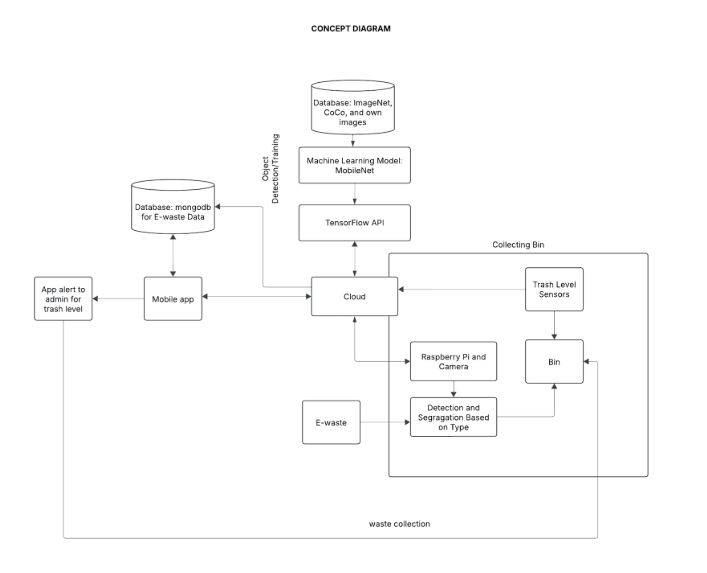
\includegraphics[width=0.5\textwidth]{Conceptual_Diagram.png}
	\caption{Proposed Conceptual Diagram}
	\label{fig:Description and Methodology}
\end{figure}

The concept diagram illustrates the research's system architecture, focusing on the backend operations of the collecting bin. At its core, the system leverages object detection and classification using a database of images, including ImageNet, CoCo, and custom datasets. MobileNet serves as the machine learning model, with TensorFlow as the API to facilitate the training process. These components are integrated into a cloud-based infrastructure, enabling seamless communication between the collecting bin and other system elements. 

The collecting bin employs IoT features, with a Raspberry Pi and camera executing the trained MobileNet model to detect and classify e-waste. Once classified, the waste is segregated and directed to the appropriate bin. Each bin is equipped with trash level sensors that monitor capacity. When the trash level reaches a predefined threshold, the sensors send a signal to the cloud, triggering notifications to the mobile app used by administrators or designated personnel.

The mobile app, connected to a MongoDB database, provides real-time trash data analytics, including bin status and alert management. Upon receiving an alert, administrators can efficiently schedule waste collection. This system ensures timely waste segregation and disposal, streamlining e-waste management and promoting sustainability. 

\textbf{Data Collection}

The data collection process for the e-waste management system is divided into backend and frontend operations to ensure efficient training, classification, and monitoring of waste disposal. 

\newline \noindent Backend Data Collection (Training and Processing)
\begin{enumerate}
	\item Image Dataset Compilation \par
The object detection and classification system leverages multiple datasets to train the MobileNet model effectively. These datasets include: 
	\begin{itemize}
		\item \textbf{ImageNet:} Provides a large-scale dataset of diverse object images for broad recognition capabilities (minimum 1000 images).
		\item \textbf{CoCo (Common Objects in Context):} Offers contextual understanding of e-waste items within various environments (minimum 1000 images).
		\item \textbf{Custom Dataset:} Includes curated images of specific e-waste items such as discarded mobile phones, circuit boards, batteries, and other electronic components (minimum 2000 images for better model adaptation to domain-specific waste).
	\end{itemize} 

These datasets undergo preprocessing, annotation, and augmentation to enhance classification accuracy. The training phase uses \textbf{TensorFlow APIs} for model optimization, ensuring high-performance detection. \newline
	
	\item Model Deployment and Cloud Integration 
	
	Once trained, the MobileNet model is deployed within a \textbf{cloud-based infrastructure} for real-time processing. The backend system performs:
	
	\begin{itemize}
		\item \textbf{Classification Processing:} Running inference on new waste images captured by the IoT-enabled bin.
		\item \textbf{Data Storage:} Storing classification results, confidence scores, and waste images in a \textbf{MongoDB database.}
		\item \textbf{Performance Monitoring:} Continuously evaluating classification accuracy and retraining the model as needed based on new data.
	\end{itemize}
\end{enumerate}

\noindent Frontend Data Collection (IoT Bins and Analytics)
\begin{enumerate}
	\item Data Collection via IoT-Enabled Collecting Bin \par

	The physical collecting bin integrates IoT components to classify and monitor waste disposal. Key features include: \begin{itemize}
	
		\item A \textbf{Raspberry Pi with a camera module} capturing images of disposed e-waste.
		\item Real-time classification of e-waste items using the deployed MobileNet model.
		\item \text{Data logging}, which records: \begin{enumerate}
			\item Timestamp of waste disposal
			\item Classified waste type
			\item Confidence score of classification
			\item Bin ID (location identifier) 
		\end{enumerate}
	\end{itemize}
	\item Trash Level Monitoring and Alerts

	 Each bin is fitted with \textbf{sensors} to track waste accumulation. The sensors provide: \begin{itemize}
		
		\item \textbf{Real-time bin capacity data}, updated at regular intervals.
		\item \textbf{Threshold alerts}, sent to the cloud system when a bin reaches its maximum capacity.
		\item \textbf{Historical disposal trends}, aiding in predictive waste management and optimized collection scheduling.
	\end{itemize}
\end{enumerate}

\textbf{Data Analysis} 
	
	The data collected from the backend machine learning model and the frontend IoT-enabled waste bins undergoes systematic analysis to enhance the efficiency of e-waste classification, optimize collection schedules, and assess the environmental impact of the system. 

\begin{enumerate}
	\item Machine Learning Model Performance Evaluation \\
To ensure the MobileNet classification model performs optimally, backend data is analyzed using:
	\begin{itemize}
		\item \textbf{Precision, Recall, and F1 Score:} Evaluate classification accuracy by measuring false positives and false negatives.
		\item \textbf{Confusion Matrix:} Visualizes misclassified e-waste items, aiding in model improvement.
		\item \textbf{Cross-Validation:} Splits the dataset into training and validation sets to assess performance across different data samples.
		\item \textbf{Retraining Frequency:} Regularly updates the dataset and retrains the model based on misclassified images to enhance accuracy.
	\end{itemize}
	\item Waste Classification Trends and Prediction \\
Frontend data collected from IoT bins helps identify e-waste disposal trends. Analytical methods include:
	\begin{itemize}
		\item \textbf{Classification Frequency Analysis:} Uses statistical aggregation to determine the most frequently disposed waste items.
		\item \textbf{Time-Series Analysis:} Forecasts future disposal rates using models such as ARIMA (AutoRegressive Integrated Moving Average).
		\item \textbf{Pattern Recognition:} Employs clustering algorithms,  K-Means to detect disposal trends and recommend bin placement adjustments.
	\end{itemize}
	\item Bin Capacity and Collection Optimization \\
Sensor data from waste bins is analyzed to optimize collection schedules such as:
	\begin{itemize}
		\item \textbf{Predictive Maintenance:} Implements machine learning algorithms to predict when bins will be full based on historical disposal rates.
	\end{itemize}
\end{enumerate}

\ifFinished
\else

\section{Estimated Work Schedule and Budget}

%The estimated work schedule can be represented as a Gantt Chart or a combination of Project Network Diagram, Work Breakdown Structure, and Critical Path.  The budget can be made into a Bill of Materials, financial plan, or if your \documentType \ is funded and part of larger project, the cost, and date for reaching each milestone and/or deliverable for your part of the project.

%For ECE Department undergraduate theses, the individual Gantt Chart or Work Breakdown Schedule and Bill of Materials will be included in this section and be removed in the final document.

%\graytx{\blindtext}

\subsection{Gantt Chart}
\FloatBarrier 
\begin{figure}[!htbp]
	\centering
		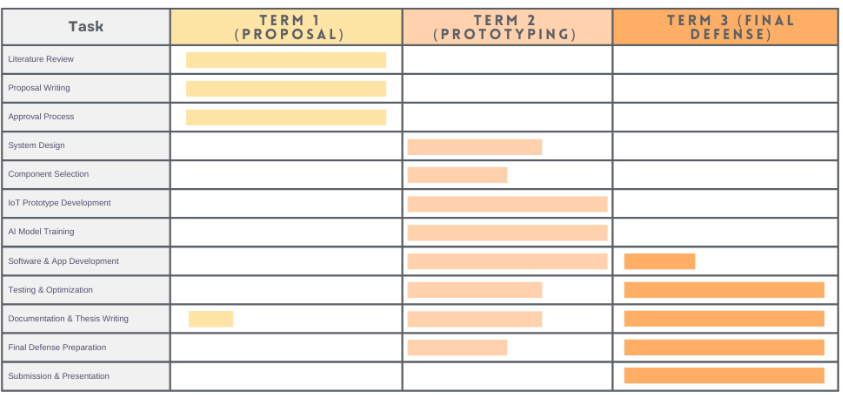
\includegraphics[width=0.5\textwidth]{Gantt_chart.png}
	\caption{Gantt Chart.}
	\label{fig:exampletc}
\end{figure}

\clearpage  % Forces everything before moving on

\subsection{Estimated Budget}

\FloatBarrier  % Ensures the Gantt chart is placed before proceeding

\begin{table}[!htbp]
    \centering
    \caption{List of Components and Costs}
    \label{tab:ComponentCosts}
    \scriptsize
    \renewcommand{\arraystretch}{1.3} % Adjusts row height
    \resizebox{\textwidth}{!}{ % Resizes table to fit page width
        \begin{tabular}{|p{0.2\textwidth}|p{0.3\textwidth}|p{0.1\textwidth}|p{0.15\textwidth}|p{0.15\textwidth}|}
            \hline
            \rowcolor[HTML]{D9D9D9} 
            \textbf{Item} & \textbf{Description} & \textbf{Quantity} & \textbf{Unit Cost} & \textbf{Total Cost} \\ 
            \hline
            \multicolumn{5}{|c|}{\textbf{Hardware}} \\ 
            \hline
            Raspberry Pi & IoT Controller & 1 & 2,215 & 2,215 \\ 
            \hline
            Ultrasonic Sensors & For bin capacity monitoring & 3 & 300 & 900 \\ 
            \hline
            Load Cells & For weight measurement & 2 & 800 & 1,600  \\ 
            \hline
            Power Supply & Adapter for IoT devices & 1 & 600 & 600 \\ 
            \hline
            \multicolumn{5}{|c|}{\textbf{Software \& Development}} \\ 
            \hline
            Cloud Hosting & Server for real-time processing & 1 Year & 470 & 5,640  \\ 
            \hline
            \multicolumn{5}{|c|}{\textbf{Testing \& Miscellaneous}} \\ 
            \hline
            Prototype Materials & Wires, PCB, casing, etc. & - & & 2,000 \\ 
            \hline
            Printing \& Documentation & Proposal, thesis, reports & - & & 1,000  \\ 
            \hline
            Contingency Fund & Unexpected expenses & - & & 1,000 \\ 
            \hline
            \multicolumn{4}{|c|}{\textbf{Total Estimated Cost}} &  14,995\\ 
            \hline
        \end{tabular}
    }
\end{table}


\ifPhD
\section{Publication Plan}
\graytx{\blindtext}
\fi

\fi


\section{Overview of the \documentType}

This chapter introduced an overview of the study, which showcases the rising issue of electronic waste (e-waste) and the necessity of an inexpensive, technologically based waste management system. The chapter detailed the history of e-waste production, health and environmental risks, and the issues arising out of improper dumping. It provided current research lacunae in waste categorization, vehicle route optimization, and user participation, emphasizing the requirement of an instantaneous Smart IoT-Inegrated Waste Management System.

The problem statement had also identified inefficiencies in current waste management operations, while the study objectives and deliverables constituted a common platform for the integration of artificial intelligence (AI), the Internet of Things (IoT), and cloud data processing for waste classification and collection improvement. The technical, social, and environmental applicability of the study was also outlined. The methodology also outlined the manner in which the system is to operate, including processes of data collection, deployment of machine learning, and integration of IoT sensors. 

Building on this context, Chapter 2: Literature Review describes literature on intelligent waste management systems today, i.e., on research that has employed deep learning, IoT, and optimisation methods for waste collection and sorting. From this chapter, various approaches will be compared, the advantages and the disadvantages of those approaches will be determined, and how this research will fill a research gap will be outlined. Readers are to anticipate discussion of contemporary technological advancements, scalability and implementational limitations, and how artificial intelligence-based methods can be utilised to improve e-waste management. From this examination, the research will position itself within the broader scholarly literature and outline its developed method.


%\stopcontents[chapters]
\cleardoublepage

%%%%%%%%%%%%%%%%%%%%%%%%%%%%%%%%%%%%%%%%%%%%%%%%
\chapter{Literature Review}
\label{ch:litrev}
%\startcontents[chapters]
%\begin{SingleSpace}	
%	\Mprintcontents 
%\end{SingleSpace}
\subsection{Literature Review}

\begin{figure}[!htbp]
	\centering
		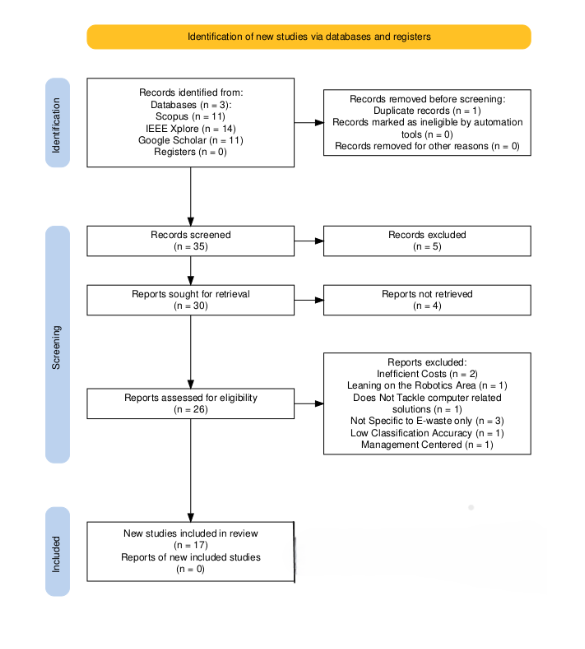
\includegraphics[width=0.5\textwidth]{PRISMA_Diagram.png}
	\caption{PRISMA Diagram}
	\label{fig:Literature Review} %?? ano bang label to
\end{figure}

The PRISMA diagram illustrates the 	systematic process that was done for selecting studies for review through screening and identification. The search identified 35 records from Scopus and IEEE Xplore along with Google Scholar though one duplicate record was excluded from the total. The evaluation of 35 records resulted in five exclusions which reduced the number of reports needed for retrieval to 30. The assessment of eligibility was reduced to 26 reports after four reports were unobtainable. The review process initiated with 35 reports but nine studies were eliminated because of respective reasons that included inefficient cost structure (2) and robot-centered research (1) while a third was considered irrelevant for computer product solutions (1). The evaluation also eliminated three studies because they lacked precision in e-waste coverage and one because of insufficient classification accuracy as well as one because it focused on management practices. The final review included 17 studies only while no new studies were reported. The methodology included specific criteria to choose only research that met the standards of relevance and quality.

\section{Existing Work}
Many studies have examined different waste management strategies, with an emphasis on the collection and disposal of e-waste. In the study of Nowakowski and Pamuła (2020), the researchers explored the use of convolutional neural networks (CNN) and Faster R-CNN for recognizing different objects, focusing specifically on improving e-waste collection strategies. While their deep learning-based system achieved an impressive classification performance of 96.7\% with CNN2, it faced challenges due to the small dataset and its sole focus on e-waste. In the study Pavan et al. (2021) conducted, a Reverse Vending Machine (RVM) that combined automation with sensors, RFID technology, and Raspberry Pi to facilitate the collection of dry and electronic waste was created. Although their innovative approach successfully promoted recycling, they encountered scalability issues tied to reliance on user participation and existing technology limitations. Similarly, Aroba et al. (2023) introduced a smart waste collection system designed for modern cities. This system leverages RFID technology and IoT-enabled sensors to monitor bin statuses in real time, aiming to enhance waste collection efficiency and improve urban cleanliness. 

Study of Nowakowski et al. (2020) improved the logistics of e-waste collection by using an AI-powered route planning system that uses the Harmony Search algorithm. The researchers' strategy effectively increased the collection efficiency, simultaneously reducing the number of vehicles required. Singh et al. (2024) developed an IoT-enabled Collector Vending Machine (CVM) for automated recycling and disposal of e-waste. The study was cost-effective but lacked thorough field testing and real-world validation. Similarly, in the study of Rani et al. in 2021, an IoT-based device, a mobile green e-waste management system for smart campuses, was created. This study were conducted to issue automated collection notifications and monitor bin levels, their concept integrated cloud-based data storage and Raspberry Pi controllers. However, the technology lacked adaptability for bigger metropolitan settings because it was designed for restricted circumstances. 

The study of Sharma et al. (2024) presented an IoT-integrated smart trash management solution that achieved a 96\% waste classification accuracy rate. Despite its effectiveness, the system's scalability in areas with limited resources was limited by the significant infrastructure investment it required. Additionally, a Smart Trash Bin model that combines spectroscopy and sensors for automated waste sorting was presented in the study of Huh et al. in 2021. The approach presented in the study uses expensive spectroscopic equipment and has trouble identifying some waste types despite its great accuracy (99.8\%). 

\section{Lacking in the Approaches}
Despite the progress in waste management research, existing studies exhibit several gaps and limitations. One significant issue is the reliance on small or specialized datasets, as observed in Nowakowski and Pamuła (2020) and Pavan et al. (2021), which restricts generalizability to real-world environments. Moreover, many studies, like studies of Singh et al. (2024) and Aroba et al. (2023), lack in extensive field validation, reducing their reliability across different geographical and socio-economic settings. Scalability remains a critical challenge, particularly in studies like Sharma et al. (2024) and Huh et al. (2021), where advanced hardware and infrastructure requirements limit implementation in low-resource regions. Furthermore, existing approaches often focus on specific waste types—such as dry waste or e-waste—without considering integrated solutions for handling mixed and bulky waste categories. This is evident in Pavan et al. (2021) and Singh et al. (2024), where proposed systems fail to accommodate broader waste management needs.

User engagement and behavior modification remain crucial yet underexplored areas. While incentive-based models like those in Pavan et al. (2021) encourage participation, studies such as Aroba et al. (2023) highlight the importance of education and accessibility in promoting sustained adoption. Without addressing these human factors, technological solutions risk underutilization and inefficiency. Additionally, hardware reliability and adaptability to real-world conditions pose additional concerns. Studies like Huh et al. (2021) and Nowakowski et al. (2020) indicate that sensor-based systems often struggle with accuracy in uncontrolled environments. Additionally, algorithmic optimizations, such as those in Nowakowski et al. (2020), tend to overlook dynamic, real-time factors like traffic conditions and fluctuating waste volumes, limiting operational efficiency.

To address these gaps, a comprehensive e-waste management system should integrate AI, IoT, and user engagement strategies while ensuring cost-effectiveness, scalability, and real-world adaptability. Addressing these limitations will enhance waste collection efficiency, optimize resource allocation, and contribute to sustainable urban and rural waste management solutions.


\section{Summary}
With this chapter, it was discovered that there have been various studies on automated waste management systems. Though a lot has been done in AI, IoT, and automation of waste collection and disposal, studies so far are still limited to some extent. The PRISMA diagram shows the systematic approach that was used in the identification of the studies, out of which the 35 initial records were narrowed down to 17 after applying the eligibility criteria.

Other studies compared robotic, IoT, and AI waste management systems. Methods like CNN-based classification (Nowakowski & Pamuła, 2020), Reverse Vending Machines (Pavan et al., 2021), and IoT-based smart bins (Sharma et al., 2024) were very efficient, with some of them having over 96% classification efficiency. The systems were not scalable, not robust to real-world testing, and not flexible. Some studies, like Singh et al. (2024) and Aroba et al. (2023), were not exposed to extensive field tests, and performance in different contexts was unknown. Others, like Huh et al. (2021), were built on costly spectroscopic hardware, and their deployment in low-resource environments was unthinkable. 

The most significant research gaps are the application of small data sets, which restrict the generalizability of machine learning models for waste segregation. Dry waste or e-waste has been addressed in most of the studies without any reference to the general issues of mixed waste management. User behavior and involvement are yet to be explored deeply, with very little intervention for long-term involvement in waste disposal programs. Studies like those of Pavan et al. (2021) used incentive models without taking into consideration overall accessibility and education for long-term adoption. These gaps can be filled by an end-to-end e-waste management system that imitates AI, IoT, and behavior interventions based on cost-effectiveness, scalability, and feasibility. Future research needs to create adaptive, data-driven solutions that enhance the efficiency of waste collection, optimize resource utilization, and promote sustainability in urban and rural settings.





%\stopcontents[chapters]
\cleardoublepage

%%%%%%%%%%%%%%%%%%%%%%%%%%%%%%%%%%%%%%%%%%%%%%%%
\chapter{Theoretical Considerations}
%\chaptermark{Theoretical Considerations} % uncomment this and put a shorter version of the chapter title for the TOC and chapter markings (i.e., header or footer)
\label{ch:theorycon}
%\startcontents[chapters]
%\begin{SingleSpace}	
%	\Mprintcontents 
%\end{SingleSpace}
Before starting the first section, provide an overview of the purpose of this chapter and its contents, and how they are relevant to your methodology.  Discuss in this chapter the relevant theories and concepts that should support your proposed solutions.

This chapter is for providing the context to your panelist/reader.  It is actually an expanded form of the Background of the Study that you have put in Chapter~\ref{ch:intro}.

\graytx{\Blindtext}

\begin{figure}[!htbp]
	\centering
		
\includegraphics[width=0.5\textwidth]{example_gray_box}
	\caption{A quadrilateral image example.}
	\label{fig:exampletc}
\end{figure}

\section{Summary}

Provide the gist of this chapter such that it reflects the contents and the message.
%\stopcontents[chapters]
\cleardoublepage

%%%%%%%%%%%%%%%%%%%%%%%%%%%%%%%%%%%%%%%%%%%%%%%%
\chapter{Design Considerations}
\label{ch:designcon}
%\startcontents[chapters]
%\begin{SingleSpace}	
%	\Mprintcontents 
%\end{SingleSpace}
Before starting the first section, provide an overview of the purpose of this chapter and its contents, and how they are relevant to your methodology. 

Your primary goal in the Design Considerations chapter is to describe to your panelist/readers the key topics that fall further under Theoretical Considerations, but should be placed here instead since they are geared towards your Methodology. These key topics are those that you have directly adopted in making your solution/methodology.  You can think of the connection of the Design Considerations chapter to the Theoretical Considerations chapter in this way: if your Theoretical Considerations chapter serves as the main foundation of a building, then the Design Considerations chapter functions as the columns. 

The  Design Considerations chapter is an avenue for explaining why you considered the topics here for your proposed methodology. This chapter is different from your methodology, because topics you discuss here are already accepted as part of the body of knowledge, and may have not been developed by you.  


\graytx{\Blindtext}

\section{Standards}

Standards are essential for successful projects and impactful research. They provide a common framework and ensure consistency, quality, and safety across various disciplines. By adhering to established standards, your work becomes more reliable, interoperable, and valuable in real-world applications. Standards also demonstrate your understanding of industry best practices and enhance the credibility of your research.

To effectively integrate standards into your project, begin by identifying relevant standards related to your specific field. Thoroughly research and understand the requirements and guidelines outlined within these standards. Align your project objectives and methodologies to meet or exceed these standards. Document your use of standards \underline{in this section}, including how and why specific standards were chosen. Finally, evaluate your results against the established standards, justifying any deviations from the norm with sound reasoning and evidence.

\section{Summary}

Provide the gist of this chapter such that it reflects the contents and message.
%\stopcontents[chapters]
\cleardoublepage

%%%%%%%%%%%%%%%%%%%%%%%%%%%%%%%%%%%%%%%%%%%%%%%%
\chapter{Methodology}
\label{ch:method}
%\startcontents[chapters]
%\begin{SingleSpace}	
%	\Mprintcontents 
%\end{SingleSpace}
Put an overview of the contents of chapter. Mention here your methodology flow through a figure and provide an overview of it and how your methodology achieves your objectives.  How your methodology achieves each of your specific objectives is what your panelists/examiners will be looking for.  Specify how your methodology achieves your general objective and specific objectives.  A point-by-point comparison how your methodology achieves each of your specific objectives is expected in the final \documentType.

Also make sure that you refer clearly to the chapters on the Literature Review, Theoretical Considerations, and Design Considerations showing how your methodology ties with those that you have discussed in those chapters.

Make an overview of the contents of the chapter. Put here your methodology flow through a figure and provide an overview of it.  


In summative form, Table~\ref{tab:methods_per_objective} indicates the approaches, designs, modes, processes, programs, techniques, and/or ways that the \documentType reaches the objectives. 


\begin{center}
	{\scriptsize
		\begin{tabularx}{\textwidth}{p{0.2\textwidth}|p{0.6\textwidth}|p{0.1\textwidth}}
			\caption{Summary of methods for reaching the objectives} \label{tab:methods_per_objective} \\
			\hline 
			\hline 
			\textbf{Objectives} & 
			\textbf{Methods} &
			\textbf{Locations}\\ 
			\hline 
			\endfirsthead
			\multicolumn{3}{c}%
			{\textit{Continued from previous page}} \\
			\hline
			\hline 
			\textbf{Objectives} & 
			\textbf{Methods} &
			\textbf{Locations}\\ 
			\hline 
			\endhead
			\hline 
			\multicolumn{3}{r}{\textit{Continued on next page}} \\ 
			\endfoot
			\hline 
			\endlastfoot
			\hline
			
			
			\Paste{GO} & \blindlist{enumerate} & Sec.~\ref{sec:implement} on p.~\pageref{sec:implement}\\ \hline
			
			
			\Paste{SO1} & \blindlist{enumerate} & Sec.~\ref{sec:implement} on p.~\pageref{sec:implement} \\ \hline
			
			
			\Paste{SO2} & \blindlist{enumerate} & Sec.~\ref{sec:implement} on p.~\pageref{sec:implement}\\ \hline
			
			
			\Paste{SO3} & \blindlist{enumerate} & Sec.~\ref{sec:implement} on p.~\pageref{sec:implement}\\ \hline
			
			
			\Paste{SO4} & \blindlist{enumerate} & Sec.~\ref{sec:implement} on p.~\pageref{sec:implement} \\ \hline
			
			
			\Paste{SO5} & \blindlist{enumerate} & Sec.~\ref{sec:implement} on p.~\pageref{sec:implement} \\ \hline
			
		\end{tabularx}
	}
\end{center}




\section{Implementation}
\label{sec:implement}

Summarize the process used to create/set-up the work with an explanation of such process, instruments, and materials that you used if any. If the description is lengthy, use condensed bullet points. 

\noindent \textit{Rule of thumb}: Implementation is how you made your  work; (keywords: implemented, created, made, soldered, programmed, etc.).

If you wrote a program or made a simulation, you must state how the program or simulation functions in this section.	An algorithm or a pseudocode as shown in Table~\ref{tab:calcxn} is a good example.


\graytx{\Blindtext}



\section{Evaluation}
\label{sec:evaluate}

Describe the procedures for evaluating the correct behavior and outcome of your  work, including what information you need to gather and how you will obtain or measure it.  

\textit{Rule of thumb}: Evaluation is how you tested your  work; (keywords: measured, tested, compared, simulated, etc.).

\graytx{\Blindtext}



\section{Summary}

Provide the gist of this chapter such that it reflects the contents and the message.

%\stopcontents[chapters]
\cleardoublepage

%%%%%%%%%%%%%%%%%%%%%%%%%%%%%%%%%%%%%%%%%%%%%%%%
\ifResultDiscuss
	\chapter{Results and Discussions}
	%	\label{ch:result_discuss} 
	%	\startcontents[chapters]
	%	\begin{SingleSpace}	
	%		\Mprintcontents 
	%	\end{SingleSpace}
	
Show in this chapter proofs why your proposed solution works.  However, presenting results ("It worked") without an appropriate explanation does not show thorough understanding.  Aside from the data and results that you have obtained, and their explanation, the discussion includes why components of your proposed solution work did or did not work in accordance to what you described in the evaluation process, and how the proposed solution performed and faired. Interpret the results and the reasons why they were obtained.  If your results are incorrect, apparent discrepancies from theory should be pointed out and explained. In essence, what do the results mean?  Citing existing publication can help you compare your results and your explanations. 

The next items below is not related to the description of this results and discussions chapter, but serves as an opener for the \LaTeX portion of this template.

Here is an example of a citation for ISO~80000-2 standard~\cite{ISO800002}. Another one is~\cite{Einstein} and~\cite{croft-78}. 

In using this template, the user is expected to have a working knowledge of \LaTeX. A good introduction is in~\cite{Oetiker2014}.  Its latest version can be accessed at \url{http://www.ctan.org/tex-archive/info/lshort}. See the Appendix of \verb|document_guide.pdf |for examples.


In aggregate form, Table~\ref{tab:outcomes_per_objective} shows the outcomes and completions in applying the methodology of the \documentType per objective. 


\begin{center}
	{\scriptsize
		\begin{tabularx}{\textwidth}{p{0.2\textwidth}|p{0.6\textwidth}|p{0.1\textwidth}}
			\caption{Summary of results for achieving the objectives} \label{tab:outcomes_per_objective} \\
			\hline 
			\hline 
			\textbf{Objectives} & 
			\textbf{Results} &
			\textbf{Locations}\\ 
			\hline 
			\endfirsthead
			\multicolumn{3}{c}%
			{\textit{Continued from previous page}} \\
			\hline
			\hline 
			\textbf{Objectives} & 
			\textbf{Results} &
			\textbf{Locations}\\ 
			\hline 
			\endhead
			\hline 
			\multicolumn{3}{r}{\textit{Continued on next page}} \\ 
			\endfoot
			\hline 
			\endlastfoot
			\hline
			
			
			\Paste{GO} & \blindlist{enumerate} & Sec.~\ref{sec:implement} on p.~\pageref{sec:implement}\\ \hline
			
			
			\Paste{SO1} & \blindlist{enumerate} & Sec.~\ref{sec:implement} on p.~\pageref{sec:implement} \\ \hline
			
			
			\Paste{SO2} & \blindlist{enumerate} & Sec.~\ref{sec:implement} on p.~\pageref{sec:implement}\\ \hline
			
			
			\Paste{SO3} & \blindlist{enumerate} & Sec.~\ref{sec:implement} on p.~\pageref{sec:implement}\\ \hline
			
			
			\Paste{SO4} & \blindlist{enumerate} & Sec.~\ref{sec:implement} on p.~\pageref{sec:implement} \\ \hline
			
			
			\Paste{SO5} & \blindlist{enumerate} & Sec.~\ref{sec:implement} on p.~\pageref{sec:implement} \\ \hline
			
		\end{tabularx}
	}
\end{center}



\graytx{\Blindtext}

\section{Summary}

Provide the gist of this chapter such that it reflects the contents and the message.
	%	\stopcontents[chapters]
	\cleardoublepage
\fi

%%%%%%%%%%%%%%%%%%%%%%%%%%%%%%%%%%%%%%%%%%%%%%%%
\ifConc
	\chapter{Conclusions, Recommendations, and Future Directives}
	\label{ch:conc}
	%	\startcontents[chapters]
	%	\begin{SingleSpace}	
	%		\Mprintcontents 
	%	\end{SingleSpace}
	\section{Concluding Remarks}

In this \documentType, \ldots

Put here the main points that should be known and learned about the  work topic. Summarize or give the gist of the essential principles and inferences drawn from your results.

\section{Contributions}

The interrelated \index{contributions} contributions and supplements that have been developed by the author(s) in this \documentType \ are listed as follows.  Only those that are unique to the authors' work are included.

\begin{itemize}
  \item the ; 
	
	\item the ; 
  
  \item the ; 
	
\end{itemize}


\section{Recommendations}

\graytx{\Blindtext}

\section{Future Prospects}

There are several prospects that may be extended for further studies. \ldots So the suggested topics are listed in the following.

\begin{enumerate}
	\item  the \ldots.
	
	\item  the \ldots.
		
	\item  the \ldots.
\end{enumerate}

Note that for ECE undergraduate theses, as per the directions of the thesis adviser, Recommendations and Future Directives will be removed for the hardbound copy but will be retained for database storage.


	%	\stopcontents[chapters]
	\cleardoublepage
\fi

%%%%%%%%%%%%%%%%%%%%%%%%%%%%%%%%%%%%%%%%%%%%%%%
\renewcommand{\UrlFont}{\normalfont}
%\bibliographystyle{IEEEtr} % for IEEE referencing format
\bibliographystyle{apalike} % for APA referencing format
\begin{SingleSpace}
	{\small \bibliography{references}}
	\vfill
	\LaTeX-comment this and the following texts after you have implemented them. See the following references for helpful guides for the bibliography and script editing in general.  Note that the links might be unavailable, but the names can be searched in the Web.

	\begin{enumerate}
		\item IEEE Citation Reference: \url{www.ieee.org/documents/ieeecitationref.pdf}

		\item IEEE Editorial Style manual: \url{www.ieee.org/documents/style_manual.pdf}

		\item IEEE Abbreviations for Transactions, Journals, Letters, and Magazines: \url{www.ieee.org/documents/trans_journal_names.pdf}
	\end{enumerate}

	\noindent Also in your BibTeX file, enclose letters or words that should all be in uppercase in curly brackets. Example: {IBM}, {P}hilippines, e{X}tensible {M}arkup {L}anguage.

\end{SingleSpace}
\vfill
\begin{flushright}
	Produced: \usdate\today, \currenttime \\
\end{flushright}
\cleardoublepage

%%%%%%%%%%%%%%%%%%%%%%%%%%%%%%%%%%%%%%%%%%%%%%%%
\SingleSpacing
\appendix
\renewcommand{\thechapter}{\Alph{chapter}}
\renewcommand{\thesection}{\thechapter\arabic{section}}
\appto\appendix{\renewcommand\thechapter{\AlphAlph{\value{chapter}}}} % for increasing appendix chapters beyond Z, i.e. AA, AB, etc.

%%%%%%%%%%%%%%%%%%%%%%%%%%%%%%%%%%%%%%%%%%%%%%%%
\chapter{Student Research Ethics Clearance}
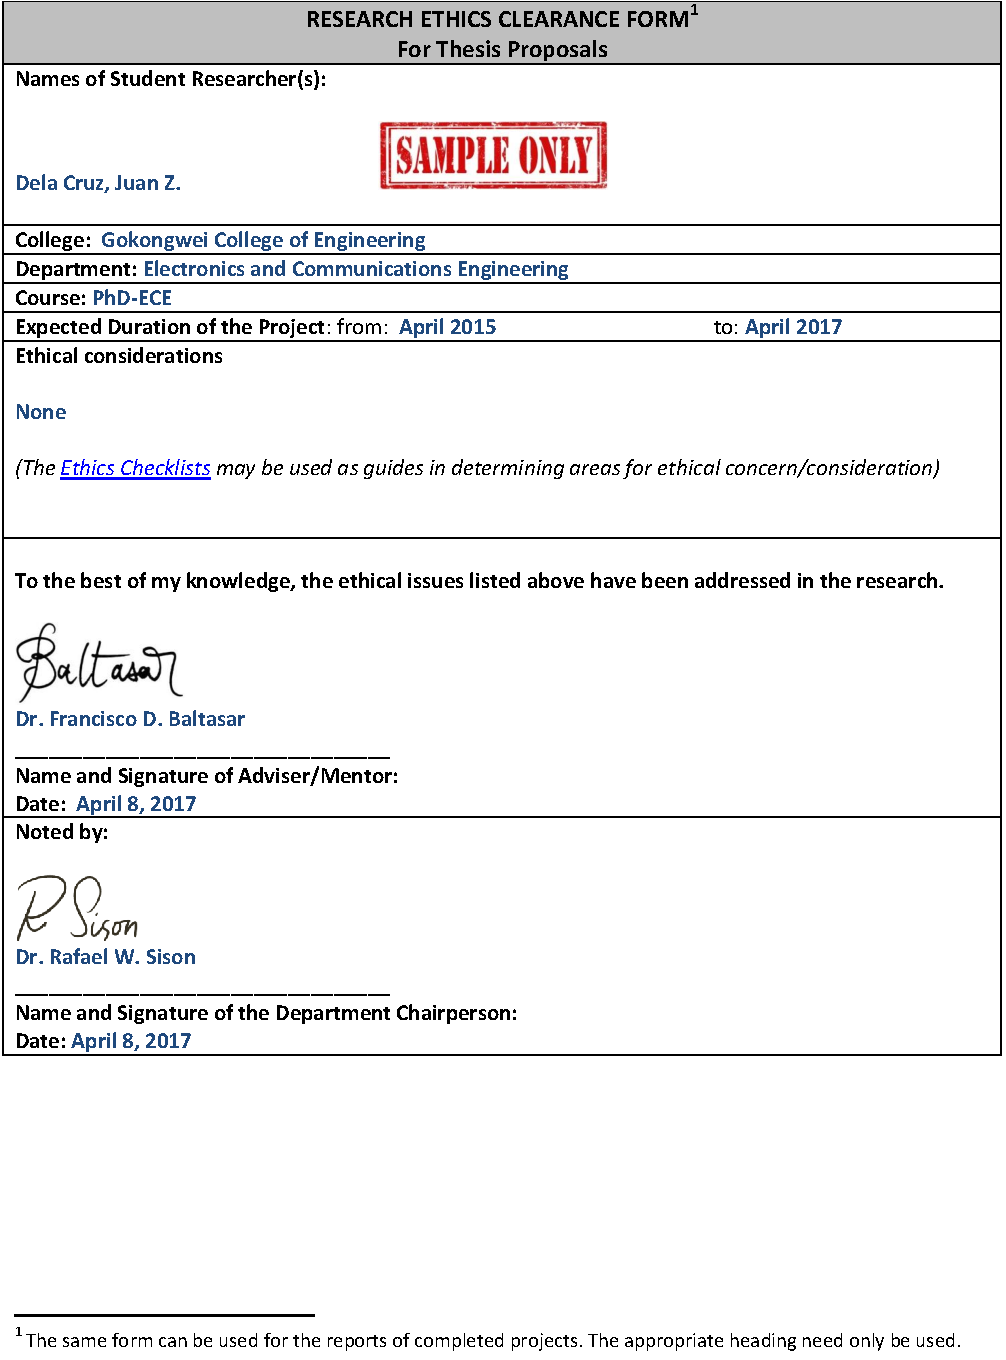
\includepdf[pages={1},%
	offset=3.5mm -10mm,%
	scale=0.75,%
	pagecommand={},]
{./figure/STUDENT_RESEARCH_ETHICS_CLEARANCE.pdf}
\cleardoublepage

%%%%%%%%%%%%%%%%%%%%%%%%%%%%%%%%%%%%%%%%%%%%%%%%
\chapter{Answers to Questions to this \documentType}
%\startcontents[chapters]
%\Mprintcontents 



\refstepcounter{section}\section*{\thesection\quad  How important is the problem to practice?}

A possible answer to this question is the summary of your Significance of the Study, and that portion of the Problem Statement where you describe the ideal scenario for your intended audience. 

\graytx{\blindtext}
	
	
	
	
\refstepcounter{section}\section*{\thesection\quad  How will you know if the solution/s that you will achieve would be better than existing ones?}	

\graytx{\blindtext}


\refstepcounter{subsection}\subsection*{\thesubsection\quad How will you measure the improvement/s?}	

\graytx{\blindtext}

	
\refstepcounter{subsubsection}\subsubsection*{\thesubsubsection\quad  What is/are your basis/bases for the improvement/s?}

\graytx{\blindtext}
	
		
\refstepcounter{subsubsection}\subsubsection*{\thesubsubsection\quad  Why did you choose that/those basis/bases?}

\graytx{\blindtext}

				
\refstepcounter{subsubsection}\subsubsection*{\thesubsubsection\quad  How significant are your measure/s of the improvement/s?}

\graytx{\blindtext}






	
\refstepcounter{section}\section*{\thesection\quad What is the difference of the solution/s from existing ones?}
	
\graytx{\blindtext}

\refstepcounter{subsection}\subsection*{\thesubsection\quad How is it different from previous and existing ones?}

\graytx{\blindtext}
	
	
	
	
	
	
\refstepcounter{section}\section*{\thesection\quad What are the assumptions made (that are behind for your proposed solution to work)?}
	
\graytx{\blindtext}
		
	
\refstepcounter{subsection}\subsection*{\thesubsection\quad Will your proposed solution/s be sensitive to these assumptions?}
	
\graytx{\blindtext}

  
\refstepcounter{subsection}\subsection*{\thesubsection\quad Can your proposed solution/s be applied to more general cases when some assumptions are eliminated? If so, how?}

\graytx{\blindtext}






\refstepcounter{section}\section*{\thesection\quad What is the necessity of your approach / proposed solution/s?}

\graytx{\blindtext}
	
	
\refstepcounter{subsection}\subsection*{\thesubsection\quad What will be the limits of applicability of your proposed~solution/s?}

\graytx{\blindtext}
				
						
\refstepcounter{subsection}\subsection*{\thesubsection\quad What will be the message of the proposed solution to technical people?  How about to non-technical managers and busines people?}
			
\graytx{\blindtext}





\refstepcounter{section}\section*{\thesection\quad How will you know if your proposed solution/s is/are correct?}

\graytx{\blindtext} 
			
			
\refstepcounter{subsection}\subsection*{\thesubsection\quad Will your results warrant the level of mathematics used (i.e., will the end justify the means)?}
	    
\graytx{\blindtext}
			





\refstepcounter{section}\section*{\thesection\quad Is/are there an/\_ alternative way/s to get to the same solution/s?}

\graytx{\blindtext}
	
	
\refstepcounter{subsection}\subsection*{\thesubsection\quad Can you come up with illustrating examples, or even better, counterexamples to your proposed solution/s?}

\graytx{\blindtext}
	
	
\refstepcounter{subsection}\subsection*{\thesubsection\quad Is there an approximation that can arrive at essentially the same proposed solution/s more easily?}
	
\graytx{\blindtext}
			
	
	
	
	
\refstepcounter{section}\section*{\thesection\quad If you were the examiner of your \documentType, how would you present the \documentType \ in another way?  Give your remarks, especially for your methodology and the results and discussions.}

% \MakeTextLowercase{\documentType} currently fails inside section{}
	
\graytx{\blindtext}
	
	
\refstepcounter{subsection}\subsection*{\thesubsection\quad What are the weaknesses of your \documentType, specifically  your methodology and the results and discussions?}

\graytx{\blindtext}

%\stopcontents[chapters]
\cleardoublepage

%%%%%%%%%%%%%%%%%%%%%%%%%%%%%%%%%%%%%%%%%%%%%%%%
\chapter{Revisions to the Proposal}
\label{ch:revisions_to_the_proposal}
%\startcontents[chapters]
%\Mprintcontents  
Make a table with the following columns for showing the summary of revisions to the proposal based on the comments of the panel of examiners. 
\begin{enumerate}
	\item  Examiner
	\item  Comment
	\item  Summary of how the comment was addressed
	\item  Locations in the document where the changes have been reflected
\end{enumerate}


\begin{center}
{\scriptsize
\begin{tabularx}{\textwidth}{p{0.1\textwidth}|p{0.2\textwidth}|p{0.5\textwidth}|p{0.1\textwidth}}
\caption{Summary of Revisions to the Proposal} \label{tab:rev_proposal} \\
\hline 
\hline 
\textbf{Examiner} & 
\textbf{Comment} & 
\textbf{Summary of how the comment was addressed} &
\textbf{Locations} \\ 
\hline 
\endfirsthead
\multicolumn{4}{c}%
{\textit{Continued from previous page}} \\
\hline
\hline 
\textbf{Examiner} & 
\textbf{Comment} & 
\textbf{Summary of how the comment was addressed} &
\textbf{Locations} \\  
\hline 
\endhead
\hline 
\multicolumn{4}{r}{\textit{Continued on next page}} \\ 
\endfoot
\hline 
\endlastfoot

\documentAdviserTitle\ \documentAdviser &
\graytx{\blindtext} &
\graytx{\blindtext \blinddescription} &
Sec.~\ref{sec:implement} on p.~\pageref{sec:implement}, Sec.~\ref{sec:evaluate} on p.~\pageref{sec:evaluate}, Fig.~\ref{fig:exampletc} on p.~\pageref{fig:exampletc}\\
\hline 

\examinerChairTitle\ \examinerChair & 
\graytx{\blindtext} &
\graytx{\blindtext \blinddescription} &
Sec.~\ref{sec:implement} on p.~\pageref{sec:implement}, Sec.~\ref{sec:evaluate} on p.~\pageref{sec:evaluate}, Fig.~\ref{fig:exampletc} on p.~\pageref{fig:exampletc}\\
\hline 

\examinerATitle\ \examinerA & 
\graytx{\blindtext} &
\graytx{\blindtext \blinditemize} &
Sec.~\ref{sec:implement} on p.~\pageref{sec:implement}, Sec.~\ref{sec:evaluate} on p.~\pageref{sec:evaluate}, Fig.~\ref{fig:exampletc} on p.~\pageref{fig:exampletc}\\
\hline 

\examinerBTitle\ \examinerB & 
\graytx{\blindtext} &
\graytx{\blindtext \blindenumerate} &
Sec.~\ref{sec:implement} on p.~\pageref{sec:implement}, Sec.~\ref{sec:evaluate} on p.~\pageref{sec:evaluate}, Fig.~\ref{fig:exampletc} on p.~\pageref{fig:exampletc}\\
\hline 

\examinerCTitle\ \examinerC & 
\graytx{\blindtext} &
\graytx{\blindtext \blindmathtrue} &
Sec.~\ref{sec:implement} on p.~\pageref{sec:implement}, Sec.~\ref{sec:evaluate} on p.~\pageref{sec:evaluate}, Fig.~\ref{fig:exampletc} on p.~\pageref{fig:exampletc}\\
\hline 

\end{tabularx}
}
\end{center}
%\stopcontents[chapters]
\cleardoublepage

%%%%%%%%%%%%%%%%%%%%%%%%%%%%%%%%%%%%%%%%%%%%%%%%
\chapter{Revisions to the Final}
\label{ch:revisions_to_the_final}
%\startcontents[chapters]
%\Mprintcontents  
Make a table with the following columns for showing the summary of revisions to the proposal based on the comments of the panel of examiners. 
\begin{enumerate}
	\item  Examiner
	\item  Comment
	\item  Summary of how the comment has been addressed
	\item  Locations in the document where the changes have been reflected
\end{enumerate}


\begin{center}
{\scriptsize
\begin{tabularx}{\textwidth}{p{0.1\textwidth}|p{0.2\textwidth}|p{0.5\textwidth}|p{0.1\textwidth}}
\caption{Summary of Revisions to the \documentType} \label{tab:rev_final} \\
\hline 
\hline 
\textbf{Examiner} & 
\textbf{Comment} & 
\textbf{Summary of how the comment has been addressed} &
\textbf{Locations} \\ 
\hline 
\endfirsthead
\multicolumn{4}{c}%
{\textit{Continued from previous page}} \\
\hline
\hline 
\textbf{Examiner} & 
\textbf{Comment} & 
\textbf{Summary of how the comment has been addressed} &
\textbf{Locations} \\  
\hline 
\endhead
\hline 
\multicolumn{4}{r}{\textit{Continued on next page}} \\ 
\endfoot
\hline 
\endlastfoot

\documentAdviserTitle\ \documentAdviser &
\graytx{\blindenumerate} &
\graytx{\blindenumerate \blinddescription} &
Sec.~\ref{sec:implement} on p.~\pageref{sec:implement}, Sec.~\ref{sec:evaluate} on p.~\pageref{sec:evaluate}, Fig.~\ref{fig:exampletc} on p.~\pageref{fig:exampletc}\\
\hline 

\examinerChairTitle\ \examinerChair & 
\graytx{\blindenumerate} &
\graytx{\blindenumerate \blinddescription} &
Sec.~\ref{sec:implement} on p.~\pageref{sec:implement}, Sec.~\ref{sec:evaluate} on p.~\pageref{sec:evaluate}, Fig.~\ref{fig:exampletc} on p.~\pageref{fig:exampletc}\\
\hline \\

\examinerATitle\ \examinerA & 
\graytx{\blindenumerate} &
\graytx{\blindenumerate \blinditemize} &
Sec.~\ref{sec:implement} on p.~\pageref{sec:implement}, Sec.~\ref{sec:evaluate} on p.~\pageref{sec:evaluate}, Fig.~\ref{fig:exampletc} on p.~\pageref{fig:exampletc}\\
\hline 

\examinerBTitle\ \examinerB & 
\graytx{\blindenumerate} &
\graytx{\blindenumerate} &
Sec.~\ref{sec:implement} on p.~\pageref{sec:implement}, Sec.~\ref{sec:evaluate} on p.~\pageref{sec:evaluate}, Fig.~\ref{fig:exampletc} on p.~\pageref{fig:exampletc}\\
\hline 

\examinerCTitle\ \examinerC & 
\graytx{\blindenumerate} &
\graytx{\blindenumerate \blindmathtrue} &
Sec.~\ref{sec:implement} on p.~\pageref{sec:implement}, Sec.~\ref{sec:evaluate} on p.~\pageref{sec:evaluate}, Fig.~\ref{fig:exampletc} on p.~\pageref{fig:exampletc}\\
\hline 

\end{tabularx}
}
\end{center}
%\stopcontents[chapters]
\cleardoublepage

%%%%%%%%%%%%%%%%%%%%%%%%%%%%%%%%%%%%%%%%%%%%%%%%
\chapter{Usage Examples}
\label{ch:usage_examples}
%\startcontents[chapters]
%\Mprintcontents  
The user is expected to have a working knowledge of \LaTeX. A good introduction is in~\cite{Oetiker2014}.  Its latest version can be accessed at \url{http://www.ctan.org/tex-archive/info/lshort}.




\section{Equations}
\label{sec:eqn_not}

The following examples show how to typeset equations in \LaTeX.  This section also shows examples of the use of \verb| \gls{ } | commands in conjunction with the items that are in the \verb| notation.tex | file. \textbf{Please make sure that the entries in} \verb| notation.tex |\textbf{  are those that are referenced in the \LaTeX \ document files used by this \documentType.  Please comment out unused notations and be careful with the commas and brackets  in} \verb| notation.tex |.

In~\eqref{eq:conv}, the output signal \gls{not:output_sigt} is the result of the convolution of the input signal \gls{not:input_sigt} and the impulse response \gls{not:ir}.

\begin{eqnarray}
	y\left( t \right) = h\left( t \right) * x\left( t \right)=\int_{-\infty}^{+\infty}h\left( t-\tau \right)x\left( \tau \right) \mathrm{d}\tau
	\label{eq:conv}
\end{eqnarray}

Other example equations are as follows.

\begin{eqnarray}
	\left[ \dfrac{ V_{1} }{ I_{1} } \right] =
	\begin{bmatrix}
		A & B \\
		C & D
	\end{bmatrix}
	\left[ \dfrac{ V_{2} }{ I_{2} } \right]
	\label{eq:ABCD}
\end{eqnarray}

\begin{eqnarray}
	\dfrac{1}{2} < \left\lfloor \mathrm{mod}\left(\left\lfloor \dfrac{y}{17} \right\rfloor 2^{-17 \lfloor x \rfloor - \mathrm{mod}(\lfloor y\rfloor, 17)},2\right)\right\rfloor,
\end{eqnarray}

\begin{eqnarray}
	| \zeta(x)^3 \zeta(x + iy)^4 \zeta(x + 2iy) | =
	\exp\sum_{n,p} \frac{3 + 4 \cos( ny \log p) + \cos (2ny \log p)}{np^{nx}} \ge 1
\end{eqnarray}

\newpage
The verbatim \LaTeX \ code of Sec.~\ref{sec:eqn_not} is in List.~\ref{lst:eqn_gls}.

\begin{lstlisting}[
float=h,
caption=Sample \LaTeX \ code for equations and notations usage, 
label=lst:eqn_gls,
language=TeX,
frame=single]
The following examples show how to typeset equations in \LaTeX.  This section also shows examples of the use of \verb| \gls{ } | commands in conjunction with the items that are in the \verb| notation.tex | file. \textbf{Please make sure that the entries in} \verb| notation.tex |\textbf{  are those that are referenced in the \LaTeX \ document files used by this \documentType.  Please comment out unused notations and be careful with the commas and brackets  in} \verb| notation.tex |.

In~\eqref{eq:conv}, the output signal \gls{not:output_sigt} is the result of the convolution of the input signal \gls{not:input_sigt} and the impulse response \gls{not:ir}.

\begin{eqnarray}   
     y\left( t \right) = h\left( t \right) * x\left( t \right)=\int_{-\infty}^{+\infty}h\left( t-\tau \right)x\left( \tau \right) \mathrm{d}\tau
	\label{eq:conv}
\end{eqnarray}

Other example equations are as follows.

\begin{eqnarray}
	\left[ \dfrac{ V_{1} }{ I_{1} } \right] = 
	\begin{bmatrix}
		A & B \\ 
		C & D 
	\end{bmatrix} 
	\left[ \dfrac{ V_{2} }{ I_{2} } \right]
	\label{eq:ABCD}
\end{eqnarray}

\begin{eqnarray}
\dfrac{1}{2} < \left\lfloor \mathrm{mod}\left(\left\lfloor \dfrac{y}{17} \right\rfloor 2^{-17 \lfloor x \rfloor - \mathrm{mod}(\lfloor y\rfloor, 17)},2\right)\right\rfloor,
\end{eqnarray}

\begin{eqnarray}
| \zeta(x)^3 \zeta(x + iy)^4 \zeta(x + 2iy) | = 
\exp\sum_{n,p} \frac{3 + 4 \cos( ny \log p) + \cos (2ny \log p)}{np^{nx}} \ge 1
\end{eqnarray}
\end{lstlisting}
\cleardoublepage







\newpage
\section{Notations}
\label{sec:not}
In order to use the standardized notation, the user is highly suggested to see the ISO~80000-2 standard~\cite{ISO800002}.

See \url{https://en.wikipedia.org/wiki/Help:Displaying_a_formula} and \url{https://en.wikipedia.org/wiki/List_of_mathematical_symbols} for \LaTeX \ maths and other notations, respectively.


The following were taken from \verb| isomath-test.tex |.

% A teststring with Latin and Greek letters::
\newcommand{\teststring}{%
	% capital Latin letters
	% A,B,C,
	A,B,
	% capital Greek letters
	%\Gamma,\Delta,\Theta,\Lambda,\Xi,\Pi,\Sigma,\Upsilon,\Phi,\Psi,
	\Gamma,\Delta,\Theta,\Lambda,\Xi,\Pi,\Sigma,\Phi,\Psi,\Omega,
	% small Greek letters
	\alpha,\beta,\pi,\nu,\omega,
	% small Latin letters:
	% compare \nu, \omega, v, and w
	v,w,
	% digits
	0,1,9
}


\subsection{Math alphabets}

If there are other symbols in place of Greek letters in a math
alphabet, it uses T1 or OT1 font encoding instead of OML.

\begin{eqnarray*}
	\mbox{mathnormal} &  & \teststring \\
	\mbox{mathit} &  & \mathit{\teststring}\\
	\mbox{mathrm} &  & \mathrm{\teststring}\\
	\mbox{mathbf} &  & \mathbf{\teststring}\\
	\mbox{mathsf} &  & \mathsf{\teststring}\\
	\mbox{mathtt} &  & \mathtt{\teststring}
\end{eqnarray*}
New alphabets bold-italic, sans-serif-italic, and sans-serif-bold-italic.
\begin{eqnarray*}
	\mbox{mathbfit}     &  & \mathbfit{\teststring}\\
	\mbox{mathsfit}     &  & \mathsfit{\teststring}\\
	\mbox{mathsfbfit} &  & \mathsfbfit{\teststring}
\end{eqnarray*}
%
Do the math alphabets match?

$
	\mathnormal  {a x \alpha \omega}
	\mathbfit    {a x \alpha \omega}
	\mathsfbfit{a x \alpha \omega}
	\quad
	\mathsfbfit{T C \Theta \Gamma}
	\mathbfit    {T C \Theta \Gamma}
	\mathnormal  {T C \Theta \Gamma}
$

\subsection{Vector symbols}

Alphabetic symbols for vectors are boldface italic,
$\vec{\lambda}=\vec{e}_{1}\cdot\vec{a}$,
while numeric ones (e.g. the zero vector) are bold upright,
$\vec{a} + \vec{0} = \vec{a}$.

\subsection{Matrix symbols}

Symbols for matrices are boldface italic, too:%
\footnote{However, matrix symbols are usually capital letters whereas vectors
	are small ones. Exceptions are physical quantities like the force
	vector $\vec{F}$ or the electrical field $\vec{E}$.%
}
$\matrixsym{\Lambda}=\matrixsym{E}\cdot\matrixsym{A}.$


\subsection{Tensor symbols}

Symbols for tensors are sans-serif bold italic,

\[
	\tensorsym{\alpha}  =  \tensorsym{e}\cdot\tensorsym{a}
	\quad \Longleftrightarrow \quad
	\alpha_{ijl}  =  e_{ijk}\cdot a_{kl}.
\]


The permittivity tensor describes the coupling of electric field and
displacement: \[
	\vec{D}=\epsilon_{0}\tensorsym{\epsilon}_{\mathrm{r}}\vec{E}\]



\newpage
\subsection{Bold math version}

The ``bold'' math version is selected with the commands
\verb+\boldmath+ or \verb+\mathversion{bold}+

{\boldmath
\begin{eqnarray*}
	\mbox{mathnormal} &  & \teststring \\
	\mbox{mathit} &  & \mathit{\teststring}\\
	\mbox{mathrm} &  & \mathrm{\teststring}\\
	\mbox{mathbf} &  & \mathbf{\teststring}\\
	\mbox{mathsf} &  & \mathsf{\teststring}\\
	\mbox{mathtt} &  & \mathtt{\teststring}
\end{eqnarray*}
New alphabets bold-italic, sans-serif-italic, and sans-serif-bold-italic.
\begin{eqnarray*}
	\mbox{mathbfit}     &  & \mathbfit{\teststring}\\
	\mbox{mathsfit}     &  & \mathsfit{\teststring}\\
	\mbox{mathsfbfit} &  & \mathsfbfit{\teststring}
\end{eqnarray*}
%
Do the math alphabets match?

$
	\mathnormal  {a x \alpha \omega}
	\mathbfit    {a x \alpha \omega}
	\mathsfbfit{a x \alpha \omega}
	\quad
	\mathsfbfit{T C \Theta \Gamma}
	\mathbfit    {T C \Theta \Gamma}
	\mathnormal  {T C \Theta \Gamma}
$

\subsubsection{Vector symbols}

Alphabetic symbols for vectors are boldface italic,
$\vec{\lambda}=\vec{e}_{1}\cdot\vec{a}$,
while numeric ones (e.g. the zero vector) are bold upright,
$\vec{a} + \vec{0} = \vec{a}$.




\subsubsection{Matrix symbols}

Symbols for matrices are boldface italic, too:%
\footnote{However, matrix symbols are usually capital letters whereas vectors
	are small ones. Exceptions are physical quantities like the force
	vector $\vec{F}$ or the electrical field $\vec{E}$.%
}
$\matrixsym{\Lambda}=\matrixsym{E}\cdot\matrixsym{A}.$


\subsubsection{Tensor symbols}

Symbols for tensors are sans-serif bold italic,

\[
	\tensorsym{\alpha}  =  \tensorsym{e}\cdot\tensorsym{a}
	\quad \Longleftrightarrow \quad
	\alpha_{ijl}  =  e_{ijk}\cdot a_{kl}.
\]

The permittivity tensor describes the coupling of electric field and
displacement: \[
	\vec{D}=\epsilon_{0}\tensorsym{\epsilon}_{\mathrm{r}}\vec{E}\]
}











\newpage
The verbatim \LaTeX \ code of Sec.~\ref{sec:not} is in List.~\ref{lst:not}.

\begin{lstlisting}[
%float=h,% do not use float option for long listings
caption=Sample \LaTeX \ code for notations usage, 
label=lst:not,
language=TeX,
frame=single]
% A teststring with Latin and Greek letters::
\newcommand{\teststring}{%
% capital Latin letters
% A,B,C,
A,B,
% capital Greek letters
%\Gamma,\Delta,\Theta,\Lambda,\Xi,\Pi,\Sigma,\Upsilon,\Phi,\Psi,
\Gamma,\Delta,\Theta,\Lambda,\Xi,\Pi,\Sigma,\Phi,\Psi,\Omega,
% small Greek letters
\alpha,\beta,\pi,\nu,\omega,
% small Latin letters:
% compare \nu, \omega, v, and w
v,w,
% digits
0,1,9
}


\subsection{Math alphabets}

If there are other symbols in place of Greek letters in a math
alphabet, it uses T1 or OT1 font encoding instead of OML.

\begin{eqnarray*}
\mbox{mathnormal} &  & \teststring \\
\mbox{mathit} &  & \mathit{\teststring}\\
\mbox{mathrm} &  & \mathrm{\teststring}\\
\mbox{mathbf} &  & \mathbf{\teststring}\\
\mbox{mathsf} &  & \mathsf{\teststring}\\
\mbox{mathtt} &  & \mathtt{\teststring}
\end{eqnarray*}
 New alphabets bold-italic, sans-serif-italic, and sans-serif-bold-italic.
\begin{eqnarray*}
\mbox{mathbfit}     &  & \mathbfit{\teststring}\\
\mbox{mathsfit}     &  & \mathsfit{\teststring}\\
\mbox{mathsfbfit} &  & \mathsfbfit{\teststring}
\end{eqnarray*}
%
Do the math alphabets match?

$
\mathnormal  {a x \alpha \omega}
\mathbfit    {a x \alpha \omega}
\mathsfbfit{a x \alpha \omega}
\quad
\mathsfbfit{T C \Theta \Gamma}
\mathbfit    {T C \Theta \Gamma}
\mathnormal  {T C \Theta \Gamma}
$

\subsection{Vector symbols}

Alphabetic symbols for vectors are boldface italic,
$\vec{\lambda}=\vec{e}_{1}\cdot\vec{a}$,
while numeric ones (e.g. the zero vector) are bold upright,
$\vec{a} + \vec{0} = \vec{a}$.

\subsection{Matrix symbols}

Symbols for matrices are boldface italic, too:%
\footnote{However, matrix symbols are usually capital letters whereas vectors
are small ones. Exceptions are physical quantities like the force
vector $\vec{F}$ or the electrical field $\vec{E}$.%
}
$\matrixsym{\Lambda}=\matrixsym{E}\cdot\matrixsym{A}.$


\subsection{Tensor symbols}

Symbols for tensors are sans-serif bold italic,

\[
   \tensorsym{\alpha}  =  \tensorsym{e}\cdot\tensorsym{a}
   \quad \Longleftrightarrow \quad
   \alpha_{ijl}  =  e_{ijk}\cdot a_{kl}.
\]


The permittivity tensor describes the coupling of electric field and
displacement: \[
\vec{D}=\epsilon_{0}\tensorsym{\epsilon}_{\mathrm{r}}\vec{E}\]



\newpage
\subsection{Bold math version}

The ``bold'' math version is selected with the commands
\verb+\boldmath+ or \verb+\mathversion{bold}+

{\boldmath
	\begin{eqnarray*}
	\mbox{mathnormal} &  & \teststring \\
	\mbox{mathit} &  & \mathit{\teststring}\\
	\mbox{mathrm} &  & \mathrm{\teststring}\\
	\mbox{mathbf} &  & \mathbf{\teststring}\\
	\mbox{mathsf} &  & \mathsf{\teststring}\\
	\mbox{mathtt} &  & \mathtt{\teststring}
	\end{eqnarray*}
	 New alphabets bold-italic, sans-serif-italic, and sans-serif-bold-italic.
	\begin{eqnarray*}
	\mbox{mathbfit}     &  & \mathbfit{\teststring}\\
	\mbox{mathsfit}     &  & \mathsfit{\teststring}\\
	\mbox{mathsfbfit} &  & \mathsfbfit{\teststring}
	\end{eqnarray*}
	%
	Do the math alphabets match?

	$
	\mathnormal  {a x \alpha \omega}
	\mathbfit    {a x \alpha \omega}
	\mathsfbfit{a x \alpha \omega}
	\quad
	\mathsfbfit{T C \Theta \Gamma}
	\mathbfit    {T C \Theta \Gamma}
	\mathnormal  {T C \Theta \Gamma}
	$

	\subsection{Vector symbols}

	Alphabetic symbols for vectors are boldface italic,
	$\vec{\lambda}=\vec{e}_{1}\cdot\vec{a}$,
	while numeric ones (e.g. the zero vector) are bold upright,
	$\vec{a} + \vec{0} = \vec{a}$.




	\subsection{Matrix symbols}

	Symbols for matrices are boldface italic, too:%
	\footnote{However, matrix symbols are usually capital letters whereas vectors
	are small ones. Exceptions are physical quantities like the force
	vector $\vec{F}$ or the electrical field $\vec{E}$.%
	}
	$\matrixsym{\Lambda}=\matrixsym{E}\cdot\matrixsym{A}.$


	\subsection{Tensor symbols}

	Symbols for tensors are sans-serif bold italic,

	\[
		 \tensorsym{\alpha}  =  \tensorsym{e}\cdot\tensorsym{a}
		 \quad \Longleftrightarrow \quad
		 \alpha_{ijl}  =  e_{ijk}\cdot a_{kl}.
	\]

	The permittivity tensor describes the coupling of electric field and
	displacement: \[
	\vec{D}=\epsilon_{0}\tensorsym{\epsilon}_{\mathrm{r}}\vec{E}\]
}

\end{lstlisting}
\cleardoublepage











\newpage
\section{Abbreviation}\
\label{sec:abbrv}

This section shows examples of the use of \LaTeX commands in conjunction with the items that are in the \verb| abbreviation.tex | and in the \verb| glossary.tex | files.  Please see List.~\ref{lst:abbrv}. \textbf{To lessen the \LaTeX \ parsing time, it is suggested that you use} \verb| \acr{ } | \textbf{only for the first occurrence of the word to be abbreviated.}

Again please see List.~\ref{lst:abbrv}. Here is an example of first use: \acr{ac}. Next use: \acr{ac}. Full: \gls{ac}.  Here's an acronym referenced using \verb| \acr |: \acr{html}.  And here it is again: \acr{html}. If you are used to the \texttt{glossaries} package, note the difference in using \verb| \gls |: \gls{html}. And again (no difference): \gls{html}. For plural use  \verb| \glspl |.  Here are some more entries:

\begin{itemize}

	\item \acr{xml} and \acr{css}.

	\item Next use: \acr{xml} and \acr{css}.

	\item Full form: \gls{xml} and \gls{css}.

	\item Reset again. \glsresetall{abbreviation}

	\item Start with a capital. \Acr{html}.

	\item Next: \Acr{html}. Full: \Gls{html}.

	\item Prefer capitals? \renewcommand{\acronymfont}[1]{\MakeTextUppercase{#1}} \Acr{xml}. Next: \acr{xml}. Full: \gls{xml}.

	\item Prefer small-caps? \renewcommand{\acronymfont}[1]{\textsc{#1}} \Acr{css}. Next: \acr{css}. Full: \gls{css}.

	\item Resetting all acronyms.\glsresetall{abbreviation}

	\item Here are the acronyms again:

	\item \Acr{html}, \acr{xml} and \acr{css}.

	\item Next use: \Acr{html}, \acr{xml} and \acr{css}.

	\item Full form: \Gls{html}, \gls{xml} and \gls{css}.

	\item Provide your own link text: \glslink{[textbf]css}{style sheet}.

\end{itemize}



The verbatim \LaTeX \ code of Sec.~\ref{sec:abbrv} is in List.~\ref{lst:abbrv}.

\begin{lstlisting}[
float=h,
caption=Sample \LaTeX \ code for abbreviations usage, 
label=lst:abbrv,
language=TeX,
frame=single]
Again please see List.~\ref{lst:abbrv}. Here is an example of first use: \acr{ac}. Next use: \acr{ac}. Full: \gls{ac}.  Here's an acronym referenced using \verb| \acr |: \acr{html}.  And here it is again: \acr{html}. If you are used to the \texttt{glossaries} package, note the difference in using \verb| \gls |: \gls{html}. And again (no difference): \gls{html}. Here are some more entries:

\begin{itemize}

	\item \acr{xml} and \acr{css}.

	\item Next use: \acr{xml} and \acr{css}.

	\item Full form: \gls{xml} and \gls{css}.

	\item Reset again. \glsresetall{abbreviation}

	\item Start with a capital. \Acr{html}.

	\item Next: \Acr{html}. Full: \Gls{html}.

	\item Prefer capitals? \renewcommand{\acronymfont}[1]{\MakeTextUppercase{#1}} \Acr{xml}. Next: \acr{xml}. Full: \gls{xml}.

	\item Prefer small-caps? \renewcommand{\acronymfont}[1]{\textsc{#1}} \Acr{css}. Next: \acr{css}. Full: \gls{css}.

	\item Resetting all acronyms.\glsresetall{abbreviation}

	\item Here are the acronyms again:

	\item \Acr{html}, \acr{xml} and \acr{css}.

	\item Next use: \Acr{html}, \acr{xml} and \acr{css}.

	\item Full form: \Gls{html}, \gls{xml} and \gls{css}.

	\item Provide your own link text: \glslink{[textbf]css}{style} 
	
\end{itemize}
\end{lstlisting}
\cleardoublepage






\newpage
\section{Glossary}
\label{sec:glos}

This section shows examples of the use of \verb| \gls{ } | commands in conjunction with the items that are in the \verb| glossary.tex | and \verb| notation.tex | files.  Note that entries in  \verb| notation.tex |  are prefixed with ``\verb| not: |'' label (see List.~\ref{lst:glos}).

\textbf{Please make sure that the entries in} \verb| notation.tex |\textbf{  are those that are referenced in the \LaTeX \ document files used by this \documentType.  Please comment out unused notations and be careful with the commas and brackets  in} \verb| notation.tex |.

\begin{itemize}

	\item \Glspl{matrix} are usually denoted by a bold capital letter, such as $\mathbfit{A}$. The \gls{matrix}'s $(i,j)$th element is usually denoted $a_{ij}$. \Gls{matrix} $\mathbf{I}$ is the identity \gls{matrix}.

	\item A set, denoted as \gls{not:set}, is a collection of objects.

	\item The universal set,  denoted as \gls{not:universalSet}, is the set of everything.

	\item The empty set, denoted as \gls{not:emptySet}, contains no elements.

	\item \Gls{Functional Analysis} is seen as the study of complete normed vector spaces, i.e., Banach spaces.

	\item The cardinality of a set, denoted as \gls{not:cardinality}, is the number of elements in the set.

\end{itemize}


The verbatim \LaTeX \ code for the part of Sec.~\ref{sec:glos} is in List.~\ref{lst:glos}.

\begin{lstlisting}[
float=h,
caption=Sample \LaTeX \ code for glossary and notations usage, 
label=lst:glos,
language=TeX,
frame=single]
\begin{itemize}

	\item \Glspl{matrix} are usually denoted by a bold capital letter, such as $\mathbfit{A}$. The \gls{matrix}'s $(i,j)$th element is usually denoted $a_{ij}$. \Gls{matrix} $\mathbf{I}$ is the identity \gls{matrix}.

	\item A set, denoted as \gls{not:set}, is a collection of objects.

	\item The universal set,  denoted as \gls{not:universalSet}, is the set of everything.

	\item The empty set, denoted as \gls{not:emptySet}, contains no elements.

	\item \Gls{Functional Analysis} is seen as the study of complete normed vector spaces, i.e., Banach spaces.
	
	\item The cardinality of a set, denoted as \gls{not:cardinality}, is the number of elements in the set.

\end{enumerate}
\end{lstlisting}
\cleardoublepage












\newpage
\section{Figure}

This section shows several ways of placing figures.  PDF\LaTeX \ compatible files are PDF, PNG, and JPG.  Please see the \verb| figure | subdirectory.

\begin{figure}[!htbp]
	\centering
	
\includegraphics[width=0.5\textwidth]{example_gray_box}
	\caption{A quadrilateral image example.}
	\label{fig:example}
\end{figure}
\cleardoublepage

Fig.~\ref{fig:example} is a gray box enclosed by a dark border. List.~\ref{lst:onefig} shows the corresponding \LaTeX \ code.


\begin{lstlisting}[
float=h,
caption=Sample \LaTeX \ code for a single figure, 
label=lst:onefig,
language=TeX,
frame=single]
\begin{figure}[!htbp]
	\centering
		\includegraphics[width=0.5\textwidth]{example}
	\caption{A quadrilateral image example.}
	\label{fig:example}
\end{figure}
\cleardoublepage

Fig.~\ref{fig:example} is a gray box enclosed by a dark border. List.~\ref{lst:onefig} shows the corresponding \LaTeX \ code. 	
\end{figure}
\end{lstlisting}
\cleardoublepage





\begin{figure}[!htbp]
	\centering
	\subbottom[A sub-figure in the top row.]{
		
\includegraphics[width=0.35\textwidth]{example_gray_box}
		\label{fig:top}
	}
	\vfill
	\subbottom[A sub-figure in the middle row.]{
		
\includegraphics[width=0.35\textwidth]{example_gray_box}
		\label{fig:mid}
	}
	\vfill
	\subbottom[A sub-figure in the bottom row.]{
		
\includegraphics[width=0.35\textwidth]{example_gray_box}
		\label{fig:botm}
	}
	\caption{Figures on top of each other. See List.~\ref{lst:figsontop} for the corresponding \LaTeX \ code. }
	\label{fig:tmb}
\end{figure}
\cleardoublepage




\begin{lstlisting}[
float=h,
caption=Sample \LaTeX \ code for three figures on top of each other, 
label=lst:figsontop,
language=TeX,
frame=single]
\begin{figure}[!htbp]
\centering
\subbottom[A sub-figure in the top row.]{

\includegraphics[width=0.35\textwidth]{example_gray_box}
\label{fig:top}
}
\vfill
\subbottom[A sub-figure in the middle row.]{

\includegraphics[width=0.35\textwidth]{example_gray_box}
\label{fig:mid}
}
\vfill
\subbottom[A sub-figure in the bottom row.]{

\includegraphics[width=0.35\textwidth]{example_gray_box}
\label{fig:botm}
}
\caption{Figures on top of each other} 
\label{fig:tmb}
\end{figure}
\end{lstlisting}
\cleardoublepage







\begin{figure}[!htbp]
	\centering
	\subbottom[A sub-figure in the upper-left corner.]{
		
\includegraphics[width=0.45\textwidth]{example_gray_box}
		\label{fig:upprleft}
	}
	\hfill
	\subbottom[A sub-figure in the upper-right corner.]{
		
\includegraphics[width=0.45\textwidth]{example_gray_box}
		\label{fig:uppright}
	}
	\vfill
	\subbottom[A sub-figure in the lower-left corner.]{
		
\includegraphics[width=0.45\textwidth]{example_gray_box}
		\label{fig:lowerleft}
	}
	\hfill
	\subbottom[A sub-figure in the lower-right corner]{
		
\includegraphics[width=0.45\textwidth]{example_gray_box}
		\label{fig:lowright}
	}
	\caption{Four figures in each corner. See List.~\ref{lst:fourfigs} for the corresponding \LaTeX \ code.}
	\label{fig:fourfig}
\end{figure}
\cleardoublepage




\begin{lstlisting}[
float=h,
caption=Sample \LaTeX \ code for the four figures, 
label=lst:fourfigs,
language=TeX,
frame=single]
\begin{figure}[!htbp]
\centering
\subbottom[A sub-figure in the upper-left corner.]{

\includegraphics[width=0.45\textwidth]{example_gray_box}
\label{fig:upprleft}
}
\hfill
\subbottom[A sub-figure in the upper-right corner.]{

\includegraphics[width=0.45\textwidth]{example_gray_box}
\label{fig:uppright}
}
\vfill
\subbottom[A sub-figure in the lower-left corner.]{

\includegraphics[width=0.45\textwidth]{example_gray_box}
\label{fig:lowerleft}
}
\hfill
\subbottom[A sub-figure in the lower-right corner]{

\includegraphics[width=0.45\textwidth]{example_gray_box}
\label{fig:lowright}
}
\caption{Four figures in each corner. See List.~\ref{lst:fourfigs} for the corresponding \LaTeX \ code.} 
\label{fig:fourfig}
\end{figure}
\end{lstlisting}
\cleardoublepage





\newpage
\section{Table}

This section shows an example of placing a table (a long one). Table~\ref{tab:triple_grid} are the triples.

\begin{center}
	{\scriptsize
		\begin{tabularx}{\textwidth}{p{0.1\textwidth}|p{0.2\textwidth}|p{0.5\textwidth}}
			\caption{Feasible triples for highly variable grid} \label{tab:triple_grid}                   \\
			\hline
			\hline
			\textbf{Time (s)}      &
			\textbf{Triple chosen} &
			\textbf{Other feasible triples}                                                               \\
			\hline
			\endfirsthead
			\multicolumn{3}{c}%
			{\textit{Continued from previous page}}                                                       \\
			\hline
			\hline
			\textbf{Time (s)}      &
			\textbf{Triple chosen} &
			\textbf{Other feasible triples}                                                               \\
			\hline
			\endhead
			\hline
			\multicolumn{3}{r}{\textit{Continued on next page}}                                           \\
			\endfoot
			\hline
			\endlastfoot
			\hline

			0                      & (1, 11, 13725) & (1, 12, 10980), (1, 13, 8235), (2, 2, 0), (3, 1, 0) \\
			2745                   & (1, 12, 10980) & (1, 13, 8235), (2, 2, 0), (2, 3, 0), (3, 1, 0)      \\
			5490                   & (1, 12, 13725) & (2, 2, 2745), (2, 3, 0), (3, 1, 0)                  \\
			8235                   & (1, 12, 16470) & (1, 13, 13725), (2, 2, 2745), (2, 3, 0), (3, 1, 0)  \\
			10980                  & (1, 12, 16470) & (1, 13, 13725), (2, 2, 2745), (2, 3, 0), (3, 1, 0)  \\
			13725                  & (1, 12, 16470) & (1, 13, 13725), (2, 2, 2745), (2, 3, 0), (3, 1, 0)  \\
			16470                  & (1, 13, 16470) & (2, 2, 2745), (2, 3, 0), (3, 1, 0)                  \\
			19215                  & (1, 12, 16470) & (1, 13, 13725), (2, 2, 2745), (2, 3, 0), (3, 1, 0)  \\
			21960                  & (1, 12, 16470) & (1, 13, 13725), (2, 2, 2745), (2, 3, 0), (3, 1, 0)  \\
			24705                  & (1, 12, 16470) & (1, 13, 13725), (2, 2, 2745), (2, 3, 0), (3, 1, 0)  \\
			27450                  & (1, 12, 16470) & (1, 13, 13725), (2, 2, 2745), (2, 3, 0), (3, 1, 0)  \\
			30195                  & (2, 2, 2745)   & (2, 3, 0), (3, 1, 0)                                \\
			32940                  & (1, 13, 16470) & (2, 2, 2745), (2, 3, 0), (3, 1, 0)                  \\
			35685                  & (1, 13, 13725) & (2, 2, 2745), (2, 3, 0), (3, 1, 0)                  \\
			38430                  & (1, 13, 10980) & (2, 2, 2745), (2, 3, 0), (3, 1, 0)                  \\
			41175                  & (1, 12, 13725) & (1, 13, 10980), (2, 2, 2745), (2, 3, 0), (3, 1, 0)  \\
			43920                  & (1, 13, 10980) & (2, 2, 2745), (2, 3, 0), (3, 1, 0)                  \\
			46665                  & (2, 2, 2745)   & (2, 3, 0), (3, 1, 0)                                \\
			49410                  & (2, 2, 2745)   & (2, 3, 0), (3, 1, 0)                                \\
			52155                  & (1, 12, 16470) & (1, 13, 13725), (2, 2, 2745), (2, 3, 0), (3, 1, 0)  \\
			54900                  & (1, 13, 13725) & (2, 2, 2745), (2, 3, 0), (3, 1, 0)                  \\
			57645                  & (1, 13, 13725) & (2, 2, 2745), (2, 3, 0), (3, 1, 0)                  \\
			60390                  & (1, 12, 13725) & (2, 2, 2745), (2, 3, 0), (3, 1, 0)                  \\
			63135                  & (1, 13, 16470) & (2, 2, 2745), (2, 3, 0), (3, 1, 0)                  \\
			65880                  & (1, 13, 16470) & (2, 2, 2745), (2, 3, 0), (3, 1, 0)                  \\
			68625                  & (2, 2, 2745)   & (2, 3, 0), (3, 1, 0)                                \\
			71370                  & (1, 13, 13725) & (2, 2, 2745), (2, 3, 0), (3, 1, 0)                  \\
			74115                  & (1, 12, 13725) & (2, 2, 2745), (2, 3, 0), (3, 1, 0)                  \\
			76860                  & (1, 13, 13725) & (2, 2, 2745), (2, 3, 0), (3, 1, 0)                  \\
			79605                  & (1, 13, 13725) & (2, 2, 2745), (2, 3, 0), (3, 1, 0)                  \\
			82350                  & (1, 12, 13725) & (2, 2, 2745), (2, 3, 0), (3, 1, 0)                  \\
			85095                  & (1, 12, 13725) & (1, 13, 10980), (2, 2, 2745), (2, 3, 0), (3, 1, 0)  \\
			87840                  & (1, 13, 16470) & (2, 2, 2745), (2, 3, 0), (3, 1, 0)                  \\
			90585                  & (1, 13, 16470) & (2, 2, 2745), (2, 3, 0), (3, 1, 0)                  \\
			93330                  & (1, 13, 13725) & (2, 2, 2745), (2, 3, 0), (3, 1, 0)                  \\
			96075                  & (1, 13, 16470) & (2, 2, 2745), (2, 3, 0), (3, 1, 0)                  \\
			98820                  & (1, 13, 16470) & (2, 2, 2745), (2, 3, 0), (3, 1, 0)                  \\
			101565                 & (1, 13, 13725) & (2, 2, 2745), (2, 3, 0), (3, 1, 0)                  \\
			104310                 & (1, 13, 16470) & (2, 2, 2745), (2, 3, 0), (3, 1, 0)                  \\
			107055                 & (1, 13, 13725) & (2, 2, 2745), (2, 3, 0), (3, 1, 0)                  \\
			109800                 & (1, 13, 13725) & (2, 2, 2745), (2, 3, 0), (3, 1, 0)                  \\
			112545                 & (1, 12, 16470) & (1, 13, 13725), (2, 2, 2745), (2, 3, 0), (3, 1, 0)  \\
			115290                 & (1, 13, 16470) & (2, 2, 2745), (2, 3, 0), (3, 1, 0)                  \\
			118035                 & (1, 13, 13725) & (2, 2, 2745), (2, 3, 0), (3, 1, 0)                  \\
			120780                 & (1, 13, 16470) & (2, 2, 2745), (2, 3, 0), (3, 1, 0)                  \\
			123525                 & (1, 13, 13725) & (2, 2, 2745), (2, 3, 0), (3, 1, 0)                  \\
			126270                 & (1, 12, 16470) & (1, 13, 13725), (2, 2, 2745), (2, 3, 0), (3, 1, 0)  \\
			129015                 & (2, 2, 2745)   & (2, 3, 0), (3, 1, 0)                                \\
			131760                 & (2, 2, 2745)   & (2, 3, 0), (3, 1, 0)                                \\
			134505                 & (1, 13, 16470) & (2, 2, 2745), (2, 3, 0), (3, 1, 0)                  \\
			137250                 & (1, 13, 13725) & (2, 2, 2745), (2, 3, 0), (3, 1, 0)                  \\
			139995                 & (2, 2, 2745)   & (2, 3, 0), (3, 1, 0)                                \\
			142740                 & (2, 2, 2745)   & (2, 3, 0), (3, 1, 0)                                \\
			145485                 & (1, 12, 16470) & (1, 13, 13725), (2, 2, 2745), (2, 3, 0), (3, 1, 0)  \\
			148230                 & (2, 2, 2745)   & (2, 3, 0), (3, 1, 0)                                \\
			150975                 & (1, 13, 16470) & (2, 2, 2745), (2, 3, 0), (3, 1, 0)                  \\
			153720                 & (1, 12, 13725) & (2, 2, 2745), (2, 3, 0), (3, 1, 0)                  \\
			156465                 & (1, 13, 13725) & (2, 2, 2745), (2, 3, 0), (3, 1, 0)                  \\
			159210                 & (1, 13, 13725) & (2, 2, 2745), (2, 3, 0), (3, 1, 0)                  \\
			161955                 & (1, 13, 16470) & (2, 2, 2745), (2, 3, 0), (3, 1, 0)                  \\
			164700                 & (1, 13, 13725) & (2, 2, 2745), (2, 3, 0), (3, 1, 0)                  \\
			\hline
		\end{tabularx}
	}
\end{center}
\cleardoublepage









List.~\ref{lst:tabl} shows the corresponding \LaTeX \ code.

\begin{lstlisting}[
%float=h,% do not use float option for long listings
caption=Sample \LaTeX \ code for making typical table environment, 
label=lst:tabl,
language=TeX,
frame=single,]
\begin{center}
{\scriptsize
\begin{tabularx}{\textwidth}{p{0.1\textwidth}|p{0.2\textwidth}|p{0.5\textwidth}}
\caption{Feasible triples for highly variable grid} \label{tab:triple_grid} \\
\hline 
\hline 
\textbf{Time (s)} & 
\textbf{Triple chosen} & 
\textbf{Other feasible triples} \\ 
\hline 
\endfirsthead
\multicolumn{3}{c}%
{\textit{Continued from previous page}} \\
\hline
\hline 
\textbf{Time (s)} & 
\textbf{Triple chosen} & 
\textbf{Other feasible triples} \\ 
\hline 
\endhead
\hline 
\multicolumn{3}{r}{\textit{Continued on next page}} \\ 
\endfoot
\hline 
\endlastfoot
\hline

0 & (1, 11, 13725) & (1, 12, 10980), (1, 13, 8235), (2, 2, 0), (3, 1, 0) \\
2745 & (1, 12, 10980) & (1, 13, 8235), (2, 2, 0), (2, 3, 0), (3, 1, 0) \\
5490 & (1, 12, 13725) & (2, 2, 2745), (2, 3, 0), (3, 1, 0) \\
8235 & (1, 12, 16470) & (1, 13, 13725), (2, 2, 2745), (2, 3, 0), (3, 1, 0) \\
10980 & (1, 12, 16470) & (1, 13, 13725), (2, 2, 2745), (2, 3, 0), (3, 1, 0) \\
13725 & (1, 12, 16470) & (1, 13, 13725), (2, 2, 2745), (2, 3, 0), (3, 1, 0) \\
16470 & (1, 13, 16470) & (2, 2, 2745), (2, 3, 0), (3, 1, 0) \\
19215 & (1, 12, 16470) & (1, 13, 13725), (2, 2, 2745), (2, 3, 0), (3, 1, 0) \\
21960 & (1, 12, 16470) & (1, 13, 13725), (2, 2, 2745), (2, 3, 0), (3, 1, 0) \\
24705 & (1, 12, 16470) & (1, 13, 13725), (2, 2, 2745), (2, 3, 0), (3, 1, 0) \\
27450 & (1, 12, 16470) & (1, 13, 13725), (2, 2, 2745), (2, 3, 0), (3, 1, 0) \\
30195 & (2, 2, 2745) & (2, 3, 0), (3, 1, 0) \\
32940 & (1, 13, 16470) & (2, 2, 2745), (2, 3, 0), (3, 1, 0) \\
35685 & (1, 13, 13725) & (2, 2, 2745), (2, 3, 0), (3, 1, 0) \\
38430 & (1, 13, 10980) & (2, 2, 2745), (2, 3, 0), (3, 1, 0) \\
41175 & (1, 12, 13725) & (1, 13, 10980), (2, 2, 2745), (2, 3, 0), (3, 1, 0) \\
43920 & (1, 13, 10980) & (2, 2, 2745), (2, 3, 0), (3, 1, 0) \\
46665 & (2, 2, 2745) & (2, 3, 0), (3, 1, 0) \\
49410 & (2, 2, 2745) & (2, 3, 0), (3, 1, 0) \\
52155 & (1, 12, 16470) & (1, 13, 13725), (2, 2, 2745), (2, 3, 0), (3, 1, 0) \\
54900 & (1, 13, 13725) & (2, 2, 2745), (2, 3, 0), (3, 1, 0) \\
57645 & (1, 13, 13725) & (2, 2, 2745), (2, 3, 0), (3, 1, 0) \\
60390 & (1, 12, 13725) & (2, 2, 2745), (2, 3, 0), (3, 1, 0) \\
63135 & (1, 13, 16470) & (2, 2, 2745), (2, 3, 0), (3, 1, 0) \\
65880 & (1, 13, 16470) & (2, 2, 2745), (2, 3, 0), (3, 1, 0) \\
68625 & (2, 2, 2745) & (2, 3, 0), (3, 1, 0) \\
71370 & (1, 13, 13725) & (2, 2, 2745), (2, 3, 0), (3, 1, 0) \\
74115 & (1, 12, 13725) & (2, 2, 2745), (2, 3, 0), (3, 1, 0) \\
76860 & (1, 13, 13725) & (2, 2, 2745), (2, 3, 0), (3, 1, 0) \\
79605 & (1, 13, 13725) & (2, 2, 2745), (2, 3, 0), (3, 1, 0) \\
82350 & (1, 12, 13725) & (2, 2, 2745), (2, 3, 0), (3, 1, 0) \\
85095 & (1, 12, 13725) & (1, 13, 10980), (2, 2, 2745), (2, 3, 0), (3, 1, 0) \\
87840 & (1, 13, 16470) & (2, 2, 2745), (2, 3, 0), (3, 1, 0) \\
90585 & (1, 13, 16470) & (2, 2, 2745), (2, 3, 0), (3, 1, 0) \\
93330 & (1, 13, 13725) & (2, 2, 2745), (2, 3, 0), (3, 1, 0) \\
96075 & (1, 13, 16470) & (2, 2, 2745), (2, 3, 0), (3, 1, 0) \\
98820 & (1, 13, 16470) & (2, 2, 2745), (2, 3, 0), (3, 1, 0) \\
101565 & (1, 13, 13725) & (2, 2, 2745), (2, 3, 0), (3, 1, 0) \\
104310 & (1, 13, 16470) & (2, 2, 2745), (2, 3, 0), (3, 1, 0) \\
107055 & (1, 13, 13725) & (2, 2, 2745), (2, 3, 0), (3, 1, 0) \\
109800 & (1, 13, 13725) & (2, 2, 2745), (2, 3, 0), (3, 1, 0) \\
112545 & (1, 12, 16470) & (1, 13, 13725), (2, 2, 2745), (2, 3, 0), (3, 1, 0) \\
115290 & (1, 13, 16470) & (2, 2, 2745), (2, 3, 0), (3, 1, 0) \\
118035 & (1, 13, 13725) & (2, 2, 2745), (2, 3, 0), (3, 1, 0) \\
120780 & (1, 13, 16470) & (2, 2, 2745), (2, 3, 0), (3, 1, 0) \\
123525 & (1, 13, 13725) & (2, 2, 2745), (2, 3, 0), (3, 1, 0) \\
126270 & (1, 12, 16470) & (1, 13, 13725), (2, 2, 2745), (2, 3, 0), (3, 1, 0) \\
129015 & (2, 2, 2745) & (2, 3, 0), (3, 1, 0) \\
131760 & (2, 2, 2745) & (2, 3, 0), (3, 1, 0) \\
134505 & (1, 13, 16470) & (2, 2, 2745), (2, 3, 0), (3, 1, 0) \\
137250 & (1, 13, 13725) & (2, 2, 2745), (2, 3, 0), (3, 1, 0) \\
139995 & (2, 2, 2745) & (2, 3, 0), (3, 1, 0) \\
142740 & (2, 2, 2745) & (2, 3, 0), (3, 1, 0) \\
145485 & (1, 12, 16470) & (1, 13, 13725), (2, 2, 2745), (2, 3, 0), (3, 1, 0) \\
148230 & (2, 2, 2745) & (2, 3, 0), (3, 1, 0) \\
150975 & (1, 13, 16470) & (2, 2, 2745), (2, 3, 0), (3, 1, 0) \\
153720 & (1, 12, 13725) & (2, 2, 2745), (2, 3, 0), (3, 1, 0) \\
156465 & (1, 13, 13725) & (2, 2, 2745), (2, 3, 0), (3, 1, 0) \\
159210 & (1, 13, 13725) & (2, 2, 2745), (2, 3, 0), (3, 1, 0) \\
161955 & (1, 13, 16470) & (2, 2, 2745), (2, 3, 0), (3, 1, 0) \\
164700 & (1, 13, 13725) & (2, 2, 2745), (2, 3, 0), (3, 1, 0) \\
\end{tabularx}
}
\end{center} 
\end{lstlisting}
\cleardoublepage













\newpage
\section{Algorithm or Pseudocode Listing}

Table~\ref{tab:calcxn} shows an example pseudocode.  Note that if the pseudocode exceeds one page, it can mean that its implementation is not modular.  List.~\ref{lst:algo} shows the corresponding \LaTeX \ code.

\begin{table}[!htbp]
	\caption{Calculation of $y = x^n$}
	\label{tab:calcxn}
	{\footnotesize
		\begin{tabular}{lll}
			\hline
			\hline
			{\bfseries Input(s):}  &   &                                     \\
			$n$                    & : & $n$th power; $n \in \mathbb{Z}^{+}$ \\
			$x$                    & : & base value; $x \in \mathbb{R}^{+}$  \\
			\hline
			{\bfseries Output(s):} &   &                                     \\
			$y$                    & : & result; $y \in \mathbb{R}^{+}$      \\
			\hline
			\hline
			\\
		\end{tabular}
	}
	\begin{algorithmic}[1]
		{\footnotesize
			\REQUIRE $n \geq 0 \vee x \neq 0$
			\ENSURE $y = x^n$
			\STATE $y \Leftarrow 1$
			\IF{$n < 0$}
			\STATE $X \Leftarrow 1 / x$
			\STATE $N \Leftarrow -n$
			\ELSE
			\STATE $X \Leftarrow x$
			\STATE $N \Leftarrow n$
			\ENDIF
			\WHILE{$N \neq 0$}
			\IF{$N$ is even}
			\STATE $X \Leftarrow X \times X$
			\STATE $N \Leftarrow N / 2$
			\ELSE[$N$ is odd]
			\STATE $y \Leftarrow y \times X$
			\STATE $N \Leftarrow N - 1$
			\ENDIF
			\ENDWHILE
		}
	\end{algorithmic}
\end{table}
\cleardoublepage




\begin{lstlisting}[
float=h,
caption=Sample \LaTeX \ code for algorithm or pseudocode listing usage, 
label=lst:algo,
language=TeX,
frame=single]
\begin{table}[!htbp]
	\caption{Calculation of $y = x^n$}
	\label{tab:calcxn}
	{\footnotesize
	\begin{tabular}{lll}
	\hline
	\hline
	{\bfseries Input(s):} & & \\
	$n$ & : & $n$th power; $n \in \mathbb{Z}^{+}$ \\
	$x$ & : & base value; $x \in \mathbb{R}^{+}$ \\
	\hline
	{\bfseries Output(s):} & & \\
	$y$ & : & result; $y \in \mathbb{R}^{+}$  \\
	\hline
	\hline
	\\
	\end{tabular}
	}
	\begin{algorithmic}[1]
	{\footnotesize
		\REQUIRE $n \geq 0 \vee x \neq 0$
		\ENSURE $y = x^n$
		\STATE $y \Leftarrow 1$
		\IF{$n < 0$}
				\STATE $X \Leftarrow 1 / x$
				\STATE $N \Leftarrow -n$
		\ELSE
				\STATE $X \Leftarrow x$
				\STATE $N \Leftarrow n$
		\ENDIF
		\WHILE{$N \neq 0$}
				\IF{$N$ is even}
						\STATE $X \Leftarrow X \times X$
						\STATE $N \Leftarrow N / 2$
				\ELSE[$N$ is odd]
						\STATE $y \Leftarrow y \times X$
						\STATE $N \Leftarrow N - 1$
				\ENDIF
		\ENDWHILE
	}	
	\end{algorithmic}
\end{table}
\end{lstlisting}
\cleardoublepage




\newpage
\section{Program/Code Listing}

List.~\ref{lst:fib_c} is a program listing of a C code for computing Fibonacci numbers by calling the actual code. Please see the \verb| code | subdirectory.

\lstinputlisting[
	float=h,
	caption={[Computing Fibonacci numbers]Computing Fibonacci numbers in C (\lstname) },
	label=lst:fib_c,
	language=C,
	frame=single]{./code/fibo.c}

List.~\ref{lst:proglist} shows the corresponding \LaTeX \ code.

\begin{lstlisting}[
float=h,
caption=Sample \LaTeX \ code for program listing, 
label=lst:proglist,
language=TeX,
frame=single]
List.~\ref{lst:fib_c} is a program listing of a C code for computing Fibonacci numbers by calling the actual code. Please see the \verb| code | subdirectory. 
\end{lstlisting}
\cleardoublepage









\newpage
\section{Referencing}
\label{sec:ref}

Referencing chapters: This appendix is in Appendix~\ref{ch:usage_examples}, which is about examples in using various \LaTeX \ commands.

Referencing sections: This section is Sec.~\ref{sec:ref}, which shows how to refer to the locations of various labels that have been placed in the \LaTeX \ files. List.~\ref{lst:refsec} shows the corresponding \LaTeX \ code.

\begin{lstlisting}[
float=h,
caption=Sample \LaTeX \ code for referencing sections, 
label=lst:refsec,
language=TeX,
frame=single]
Referencing sections: This section is Sec.~\ref{sec:ref}, which shows how to refer to the locations of various labels that have been placed in the \LaTeX \ files. List.~\ref{lst:refsec} shows the corresponding \LaTeX \ code.  
\end{lstlisting}
\graytx{\blindtext}
\cleardoublepage






\subsection{A subsection}
\label{sec:subsec}

Referencing subsections: This section is Sec.~\ref{sec:subsec}, which shows how to refer to a subsection. List.~\ref{lst:refsub} shows the corresponding \LaTeX \ code.

\begin{lstlisting}[
float=h,
caption=Sample \LaTeX \ code for referencing subsections, 
label=lst:refsub,
language=TeX,
frame=single]
Referencing subsections: This section is Sec.~\ref{sec:subsec}, which shows how to refer to a subsection. List.~\ref{lst:refsub} shows the corresponding \LaTeX \ code. 
\end{lstlisting}
\graytx{\blindtext}
\cleardoublepage





\subsubsection{A sub-subsection}
\label{sec:subsubsec}


Referencing sub-subsections: This section is Sec.~\ref{sec:subsubsec}, which shows how to refer to a sub-subsection.  List.~\ref{lst:refsubsub} shows the corresponding \LaTeX \ code.

\begin{lstlisting}[
float=h,
caption=Sample \LaTeX \ code for referencing sub-subsections, 
label=lst:refsubsub,
language=TeX,
frame=single]
Referencing sub-subsections: This section is Sec.~\ref{sec:subsubsec}, which shows how to refer to a sub-subsection. List.~\ref{lst:refsubsub} shows the corresponding \LaTeX \ code. 
\end{lstlisting}

\graytx{\blindtext}
\cleardoublepage





\newpage
\section{Citing}
\label{sec:cit}

Citing bibliography content is done using BibTeX. It requires the creation of a BibTeX file~(.bib extension name), and then added in the argument of \verb| \bibliography{ } |. For each .bib file, separate them by a comma in the argument of \verb| \bibliography{ } | without the extension name. Building your BibTeX file~(references.bib) can be done easily with a tool called JabRef~(\url{www.jabref.org}).

The following subsections are examples of citations.

%\begin{multicols}{2}

\subsection{Books}
\begin{itemize}
	\item \cite{chicago-82}
	\item \cite{aristotle:rhetoric}
	\item \cite{aristotle:anima}
	\item \cite{aristotle:poetics}
	\item \cite{aristotle:physics}
	\item \cite{BCM-59}
	\item \cite{augustine}
	\item \cite{averroes/bland}
	\item \cite{butcher-81}
	\item \cite{chapman-75}
	\item \cite{cicero}
	\item \cite{coleridge}
	\item \cite{cotton}
	\item \cite{vangennep}
	\item \cite{vangennep:related}
	\item \cite{vangennep:trans}
	\item \cite{gerhardt}
	\item \cite{gonzalez}
	\item \cite{companion}
	\item \cite{hammond}
	\item \cite{hershkovitz-62}
	\item \cite{hoel-71-whole}
	\item \cite{iliad}
	\item \cite{book-full}
	\item \cite{book-minimal}
	\item \cite{whole-set}
	\item \cite{kullback:related}
	\item \cite{kullback:reprint}
	\item \cite{kullback}
	\item \cite{malinowski}
	\item \cite{maron}
	\item \cite{massa}
	\item \cite{mccolvin-nodate}
	\item \cite{nietzsche:ksa}
	\item \cite{nietzsche:ksa1}
	\item \cite{Oetiker2014}
	\item \cite{piccato}
	\item \cite{smart-76}
	\item \cite{vazques-de-parga}
	\item \cite{wilde}
	\item \cite{wood-61}
	\item \cite{worman}
	\item \cite{wright-78-book}
	\item \cite{whole-collection}
\end{itemize}



\subsection{Booklets}
\begin{itemize}
	\item \cite{booklet-full}
\end{itemize}


\subsection{Proceedings}
\begin{itemize}
	\item \cite{proceedings-full}
\end{itemize}


\subsection{In books}
\begin{itemize}
	\item \cite{brandt}
	\item \cite{bs-2570-inbook}
	\item \cite{eckstein-zuckerman}
	\item \cite{feigl-58}
	\item \cite{gordon-75}
	\item \cite{hanson-67}
	\item \cite{hoel-71-portion}
	\item \cite{hyman}
	\item \cite{kant:kpv}
	\item \cite{kant:ku}
	\item \cite{inbook-full}
	\item \cite{inbook-minimal}
	\item \cite{incollection-full}
	\item \cite{incollection-crossref}
	\item \cite{incollection-minimal}
	\item \cite{mcneill-63}
	\item \cite{milton-24}
	\item \cite{nietzsche:historie}
	\item \cite{ogilvy-65}
	\item \cite{pines}
	\item \cite{ramsbottom-31}
	\item \cite{ranganathan-51}
	\item \cite{thomson-71}
	\item \cite{wright-63}
	\item \cite{wright-78-incollection}
\end{itemize}



\subsection{In proceedings}
\begin{itemize}
	\item \cite{chave-64}
	\item \cite{chomsky-73}
	\item \cite{moraux}
	\item \cite{inproceedings-full}
	\item \cite{inproceedings-crossref}
	\item \cite{inproceedings-minimal}
	\item \cite{salam}
\end{itemize}




\subsection{Journals}

\begin{itemize}
	\item \cite{article-crossref}
	\item \cite{article-full}
	\item \cite{article-minimal}
	\item \cite{aksin}
	\item \cite{angenendt}
	\item \cite{aslin-49}
	\item \cite{baez/article}
	\item \cite{bertram}
	\item \cite{bry-afflerbach}
	\item \cite{doody}
	\item \cite{Einstein}
	\item \cite{fletcher-hopkins}
	\item \cite{gillies}
	\item \cite{glashow}
	\item \cite{godfrey-59}
	\item \cite{hanlon-72}
	\item \cite{heller-lederis}
	\item \cite{herrmann}
	\item \cite{murray}
	\item \cite{howells-66-pop}
	\item \cite{howells-66-var}
	\item \cite{howells-51}
	\item \cite{ISO800002}
	\item \cite{jackson-79}
	\item \cite{johnson-74}
	\item \cite{moore:related}
	\item \cite{moore}
	\item \cite{prufer-64}
	\item \cite{reese}
	\item \cite{sarfraz}
	\item \cite{shore}
	\item \cite{sigfridsson}
	\item \cite{weinberg}
	\item \cite{yoon}
	\item \cite{whole-journal}
\end{itemize}





\subsection{Theses/dissertations}
\begin{itemize}
	\item \cite{croft-78}
	\item \cite{maguire-76}
	\item \cite{mann-68}
	\item \cite{mastersthesis-full}
	\item \cite{mastersthesis-minimal}
	\item \cite{phdthesis-full}
	\item \cite{phdthesis-minimal}
\end{itemize}


\subsection{Technical Reports and Others}
\begin{itemize}
	\item \cite{brunswick-85}
	\item \cite{bs-6371}
	\item \cite{bs-5605}
	\item \cite{bs-1629}
	\item \cite{bs-2570-techreport}
	\item \cite{ellis-walton}
	\item \cite{techreport-full}
	\item \cite{techreport-minimal}
	\item \cite{winget-67}
	\item \cite{unpublished-minimal}
	\item \cite{unpublished-full}
	\item \cite{downes-74}
	\item \cite{exchequer-34-39}
	\item \cite{pym-24}
	\item \cite{traquair-38}
\end{itemize}


\subsection{Miscellaneous}
\begin{itemize}
	\item \cite{almendro}
	\item \cite{baez/online}
	\item \cite{chiu}
	\item \cite{itzhaki}
	\item \cite{kowalik}
	\item \cite{laufenberg}
	\item \cite{loh}
	\item \cite{markey}
	\item \cite{misc-full}
	\item \cite{padhye}
	\item \cite{sorace}
	\item \cite{wassenberg}
	\item \cite{misc-minimal}
\end{itemize}


%\end{multicols}

\cleardoublepage









\newpage
\section{Index}

For key words or topics that are expected (or the user would like) to appear in the Index, use \verb| index{key} |, where  \verb| key | is an example keyword to appear in the Index. For example, Fredholm integral and Fourier operator of the following paragraph are in the Index.

If we make a very large matrix with complex exponentials in the rows (i.e., cosine real parts and sine imaginary parts), and increase the resolution without bound, we approach the kernel of the \index{Fredholm integral} Fredholm integral equation of the 2nd kind, namely the \index{Fourier operator} Fourier operator that defines the continuous Fourier transform.

List.~\ref{lst:indxsample} is a program listing of the above-mentioned paragraph.

\begin{lstlisting}[
float=h,
caption=Sample \LaTeX \ code for Index usage, 
label=lst:indxsample,
language=TeX,
frame=single]
If we make a very large matrix with complex exponentials in the rows (i.e., cosine real parts and sine imaginary parts), and increase the resolution without bound, we approach the kernel of the \index{Fredholm integral} Fredholm integral equation of the 2nd kind, namely the \index{Fourier} Fourier operator that defines the continuous Fourier transform.
\end{lstlisting}
\cleardoublepage




\newpage
\section{Adding Relevant PDF Pages}

Examples of such PDF pages are Standards, Datasheets, Specification Sheets, Application Notes, etc.  Selected PDF pages can be added (see List.~\ref{lst:pdfpages}), but note that the options must be tweaked.  See the manual of \verb| pdfpages | for other options.

\begin{lstlisting}[
float=h,
caption=Sample \LaTeX \ code for including PDF pages, 
label=lst:pdfpages,
language=TeX,
frame=single]
\includepdf[pages={8-10},%
offset=3.5mm -10mm,%
scale=0.73,%
frame,%
pagecommand={},]
{./reference/Xilinx2015-UltraScale-Architecture-Overview.pdf}
\end{lstlisting}
\cleardoublepage

\includepdf[pages={8-10},%
	offset=3.5mm -10mm,%
	scale=0.73,%
	frame,%
	pagecommand={},]
{./reference/Xilinx2015-UltraScale-Architecture-Overview.pdf}
%\stopcontents[chapters]
\cleardoublepage

%%%%%%%%%%%%%%%%%%%%%%%%%%%%%%%%%%%%%%%%%%%%%%%%
\chapter{Some List of Math Symbols}
\label{ch:math_sym}

\includepdf[pages={1-17},%
	offset=3.5mm -10mm,%
	scale=0.74,%
	%frame,%
	pagecommand={},]
{../../List-of-mathematical-symbols.pdf}
\cleardoublepage

%%%%%%%%%%%%%%%%%%%%%%%%%%%%%%%%%%%%%%%%%%%%%%%%
\chapter{Dislaying Math Expressions}
\label{ch:disp_math}

\includepdf[pages={1-31},%
	offset=3.5mm -10mm,%
	scale=0.74,%
	%frame,%
	pagecommand={},]
{../../Help-Displaying-a-formula.pdf}
\cleardoublepage

%%%%%%%%%%%%%%%%%%%%%%%%%%%%%%%%%%%%%%%%%%%%%%%%
\chapter{IEEE Editorial Style Manual}
\label{ch:ieee_edsm}

\includepdf[pages={1-31},%
	offset=3.5mm -10mm,%
	scale=0.74,%
	%frame,%
	pagecommand={},]
{../../IEEE-Editorial-Style-manual.pdf}
\cleardoublepage

%%%%%%%%%%%%%%%%%%%%%%%%%%%%%%%%%%%%%%%%%%%%%%%%
\chapter{IEEE Citation Reference}
\label{ch:ieee_cr}

\includepdf[pages={1-7},%
	offset=3.5mm -10mm,%
	scale=0.75,%
	%frame,%
	pagecommand={},]
{../../IEEE-Citation-Reference.pdf}
\cleardoublepage

%%%%%%%%%%%%%%%%%%%%%%%%%%%%%%%%%%%%%%%%%%%%%%%%
\chapter{IEEE Publication Abbreviations}
\label{ch:ieee_pub_abb}

\includepdf[pages={1-7},%
	offset=3.5mm -10mm,%
	scale=0.73,%
	%frame,%
	pagecommand={},]
{../../IEEE-Abbreviations-for-Transactions-Journals-Letters-and-Magazines.pdf}
\cleardoublepage

%%%%%%%%%%%%%%%%%%%%%%%%%%%%%%%%%%%%%%%%%%%%%%%%
\chapter{IEEE Index Terms}
\label{ch:ieee_keywords}

\includepdf[pages={1-67},%
	offset=3.5mm -10mm,%
	scale=0.75,%
	%frame,%
	pagecommand={},]
{../../IEEE-taxonomy-v101.pdf}
\cleardoublepage

%%%%%%%%%%%%%%%%%%%%%%%%%%%%%%%%%%%%%%%%%%%%%%%%
\ifPubList
	\chapter{Publication List and Award}

\flushleft{\Large \bfseries Journal (example only)\\}

\begin{enumerate}
\item \href{http://10.1016/j.jorganchem.2006.03.012}{{\"O}.~Aks{\i}n, H.~T{\"u}rkmen, \textbf{L.~Artok}, B.~{\c{C}}etinkaya, C.~Ni, 
  O.~B{\"u}y{\"u}kg{\"u}ng{\"o}r, and E.~{\"O}zkal, ``Effect of immobilization
  on catalytic characteristics of saturated pd-n-heterocyclic carbenes in
  mizoroki-heck reactions,'' {\em Journal of Organometallic Chemistry},
  vol.~691, no.~13, pp.~3027--3036, 2006.}

\item \ldots

\end{enumerate}
\vspace{2ex}


\flushleft{\Large \bfseries Monograph\\}

\begin{enumerate}

\item \ldots

\item \ldots

\end{enumerate}
\vspace{2ex}



\flushleft{\Large \bfseries Conference}\\
\begin{enumerate}

\item \ldots

\item \ldots

\end{enumerate}
\vspace{2ex}



\flushleft{\Large \bfseries Award}\\

\begin{enumerate}
\item \ldots

\item \ldots
\end{enumerate}
\fi
\cleardoublepage

%%%%%%%%%%%%%%%%%%%%%%%%%%%%%%%%%%%%%%%%%%%%%%%%
\ifVita
	\chapter{Vita}

% Change the descriptions accordingly

\foreach \n in {1,...,\numberOfAuthors}{
\vfill

\includegraphics[width=0.2\columnwidth]{vita_photo}
\documentAuthor{firstname\n} \ \documentAuthor{surname\n} \ received the B.Sc., M.Sc., and Ph.D. degrees in chemistry all from the Pamantasan ng Pilipinas, San~Juan, Metro~Manila, Philippines, in {\xinttheiexpr \xintexpr \the\year - 5 \relax \relax}, {\xinttheiexpr \xintexpr \the\year - 3 \relax \relax} and \the\year \ respectively. He is currently taking up his B.Sc. \degree \ studies.  He has developed several high-speed packet-switched network systems and node modules. His research interests include high-speed packet-switched networks, high speed radio interface design, discrete simulation and statistical models for packet switches.

\vfill
}
\fi
\cleardoublepage

%%%%%%%%%%%%%%%%%%%%%%%%%%%%%%%%%%%%%%%%%%%%%%%%
\ifIndex
	\printindex
\fi

%%%%%%%%%%%%%%%%%%%%%%%%%%%%%%%%%%%%%%%%%%%%%%%%
\chapter{Article Paper(s)}
\label{ch:article_paper}
\cleardoublepage
{
	\ClearWallPaper
	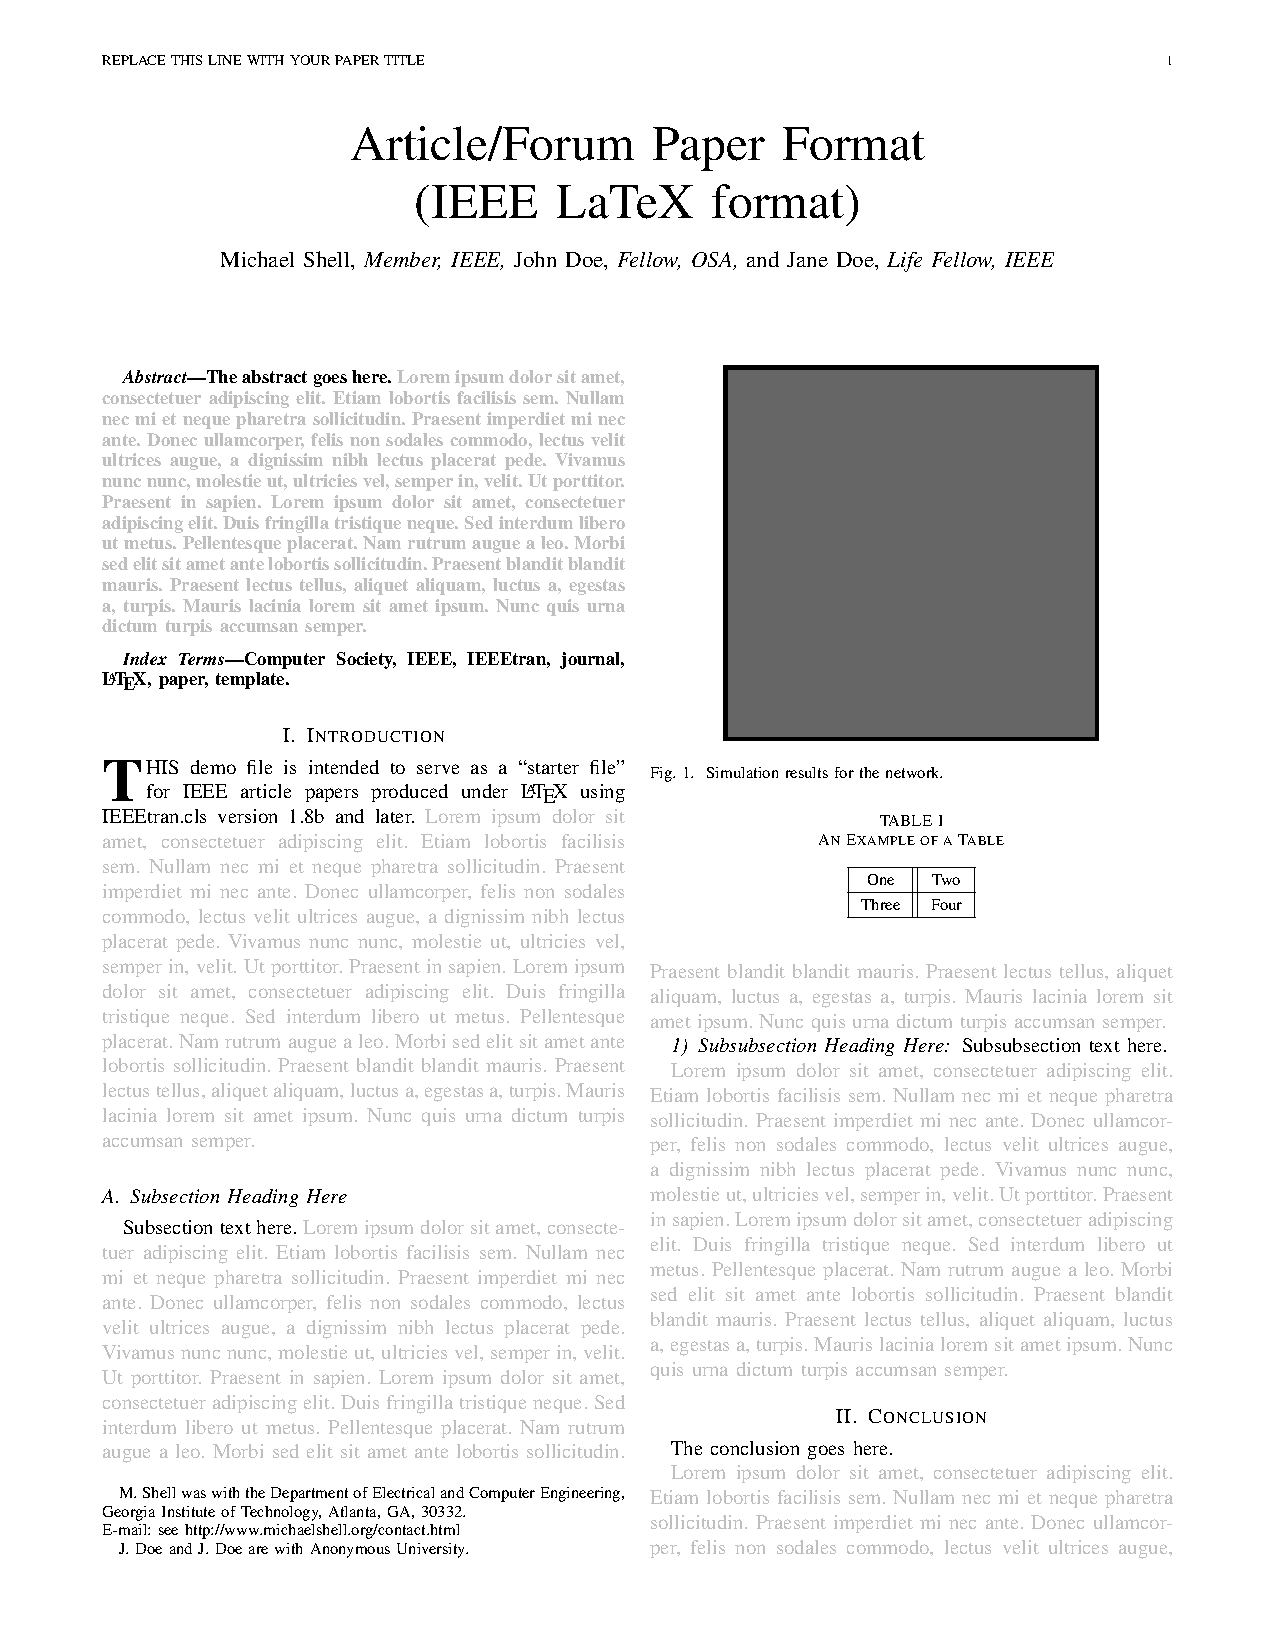
\includepdf[pages=-,%
		scale=1.0,%
		frame,%
	]
	{article_forum_paper.pdf}
}
\cleardoublepage

\end{document}